

\section{IndianSuburb-5K: Data and SAM3-Only Annotation Plan}
\label{sec:indiasuburb5k_data}

\paragraph{Motivation.}
To study whether video world-models trained predominantly on Western web data transfer to Indian suburb street ecology, we construct \textbf{IndianSuburb-5K}, a dataset of \textbf{5,000} long-form YouTube videos curated to emphasize \textbf{(i) narrow mixed-traffic roads} (pedestrians, bikes, autos, animals; informal lane discipline) and \textbf{(ii) street markets} (dense occlusion, signage clutter, high interaction intensity). The dataset is designed to support \emph{label-free} and \emph{annotation-light} evaluation of representation learning and predictive modeling under domain shift. Since manual labeling at scale is infeasible, our annotation pipeline is \textbf{fully automatic} and uses \textbf{SAM3} as the sole annotation engine for instance masks and tracking, from which we derive scene difficulty, interaction structure, and factorized supervision signals.

\subsection{Data Collection and Curation}
\label{sec:indiasuburb5k_collection}

\paragraph{Source and inclusion criteria.}
We collect long-form public videos from YouTube (e.g., walking tours, handheld POV, dashcam drives) depicting \textbf{Indian suburban streets} and \textbf{open markets}. We prioritize continuous footage with minimal cuts, natural motion, and realistic density (rather than cinematic edits). Each source video is stored only as a reference identifier with timestamps unless the license explicitly permits redistribution.

\paragraph{Scene taxonomy (primary pillars).}
Each source video is assigned one primary pillar and up to two secondary modifiers:
\begin{itemize}[leftmargin=*,itemsep=2pt]
  \item \textbf{P1: Narrow mixed-traffic roads} (heterogeneous agents, frequent merges/crossings, unmarked lanes).
  \item \textbf{P2: Street markets} (dense crowds, stalls, signage clutter, frequent occlusions).
  \item \textbf{P0: Low-density suburb lanes (control)} (gated/residential lanes; low interaction intensity) to ensure baseline comparability.
  \item \textbf{Modifiers:} night/low-light, rain/monsoon, construction, high-signage, animals-present (when detectable), high-occlusion.
\end{itemize}

\paragraph{Clipification.}
World-model evaluation operates on clips, not full videos. We standardize each source into fixed-length clips: duration $T\in[8,16]$ seconds (default $T=8$s), FPS $f\in\{12,15\}$ (default 12), and normalized resolution (short-side 384 or 512). Clips are extracted with stride $s$ (e.g., one clip every 20--30 seconds of source time) to reduce near-duplicates and ensure coverage. Each clip is uniquely identified by $(\texttt{video\_id}, t_{\mathrm{start}}, t_{\mathrm{end}})$ and stored as a path in the manifest.

\paragraph{Quality filtering and de-duplication.}
We automatically remove non-informative or confounded segments: (i) extremely low motion (static shots, slides), (ii) heavy overlays (large captions, split-screens), (iii) indoor segments, and (iv) extreme blur. Near-duplicate clips are pruned both within and across videos using perceptual hashing on keyframes and embedding similarity on a lightweight video encoder (thresholded to preserve diversity while retaining intra-scene variation). The dedup stage is essential for self-supervised evaluation, where duplicates can artificially inflate apparent generalization.

\subsection{SAM3-Only Annotation Pipeline}
\label{sec:indiasuburb5k_sam3}

\paragraph{Design principle.}
SAM3 provides instance masks; we treat all higher-level labels as \textbf{derived} from masks and their temporal association. This yields a scalable, reproducible pipeline that supports factorized evaluation (layout, agents, interactions) without any manual bounding boxes or dense labeling.

\paragraph{Per-frame segmentation and temporal association.}
For each clip, SAM3 produces per-frame instance masks $\{m_{t}^{(k)}\}_{k=1}^{K_t}$ and confidences. We associate masks across time to form tracklets $\tau^{(u)}=\{m_{t}^{(u)}\}_{t\in \mathcal{T}_u}$ via mask IoU + motion consistency (or SAM3 tracking mode when available). Each tracklet stores mask area, centroid trajectory, and velocity estimates. We compute track fragmentation and ID switches as indicators of occlusion and scene difficulty.

\paragraph{Derived scene statistics (clip-level).}
From masks and tracklets we compute a compact set of clip-level statistics used for (i) stratified evaluation, (ii) stress-test subsets, and (iii) automatic pseudo-labels:
\begin{itemize}[leftmargin=*,itemsep=2pt]
  \item \textbf{Agent density} $D$: mean/peak number of instances per frame; $D=\mathbb{E}_t[K_t]$, $D_{\max}=\max_t K_t$.
  \item \textbf{Clutter ratio} $C$: fraction of pixels covered by instance masks, $C=\mathbb{E}_t\left[\frac{\sum_k |m_t^{(k)}|}{|\Omega|}\right]$.
  \item \textbf{Occlusion index} $O$: mean pairwise overlap of masks plus track fragmentation, $O=\mathbb{E}_t\left[\sum_{i\neq j}\frac{|m_t^{(i)}\cap m_t^{(j)}|}{|m_t^{(i)}\cup m_t^{(j)}|}\right] + \lambda\,\mathrm{Frag}$.
  \item \textbf{Interaction proximity} $P$: number of close-approach events between track centroids (distance below threshold for at least $k$ frames), optionally normalized by agent count.
  \item \textbf{Motion intensity} $M$: optical-flow magnitude statistics (computed automatically; not a human label) used only for matching controls.
  \item \textbf{Visibility proxies} $V$: brightness/contrast and blur measures to create day/night and low-visibility subsets.
\end{itemize}

\paragraph{SAM3 Difficulty Index (SDI).}
We collapse the above into a single scalar difficulty axis to enable simple, interpretable robustness plots:
\begin{equation}
\label{eq:sdi}
\mathrm{SDI} \;=\; \alpha\,\widetilde{D} \;+\; \beta\,\widetilde{O} \;+\; \gamma\,\widetilde{C} \;+\; \delta\,\widetilde{P} \;+\; \eta\,\widetilde{\mathrm{Frag}},
\end{equation}
where $\widetilde{\cdot}$ denotes min--max normalized statistics within the training partition. We set $(\alpha,\beta,\gamma,\delta,\eta)$ once on a development subset and keep fixed thereafter. SDI enables a single headline curve: world-model error vs.\ scene difficulty (easy $\rightarrow$ hard) with confidence intervals.

\subsection{Factorized Supervision: Layout, Agents, Interactions}
\label{sec:indiasuburb5k_factorized}

\paragraph{Why factorization.}
To diagnose \emph{what} transfers and \emph{what} fails, we define three factor views aligned with the model-agnostic decomposition: \textbf{layout} (static geometry), \textbf{agents} (who/where), and \textbf{interactions} (how they relate). All targets are derived automatically from SAM3 outputs, enabling layerwise probe evaluation.

\paragraph{Layout stream (static structure).}
We create a layout-centric representation by suppressing dynamic instances: for each frame, we remove (mask-out) SAM3 instances and retain the complement region as a proxy for background layout. We optionally compute coarse regions (road-like vs non-road-like) via unsupervised clustering over background textures and motion cues; these are treated as \emph{soft} targets, used only for relative comparisons. The layout stream supports tasks such as background reconstruction consistency, static region stability, and layout accessibility across depth.

\paragraph{Agents stream (instance-centric).}
We create agent-centric frames retaining only SAM3 instance regions. Since SAM3 does not natively classify categories, our primary supervision is \textbf{category-free}: instance density maps, per-frame counts, size/shape histograms, and track motion statistics. We also report a \textbf{heterogeneity index} $H$ capturing the diversity of instance scale and motion (useful as a proxy for mixed traffic):
\begin{equation}
\label{eq:heterogeneity}
H \;=\; \mathrm{Entropy}\big(\mathrm{bin}(\mathrm{area}) \times \mathrm{bin}(\mathrm{speed}) \times \mathrm{bin}(\mathrm{aspect})\big).
\end{equation}
High $H$ strongly correlates with heterogeneous streets even without explicit semantic labels.

\paragraph{Interactions stream (geometry + dynamics).}
We represent interactions as a time-indexed graph over tracklets. For tracklets $u,v$ at time $t$, we define edge features such as centroid distance, relative velocity, and overlap. A clip-level interaction tensor aggregates: (i) number of close-approach events, (ii) duration of proximity, and (iii) ordering swaps along the dominant motion axis (a proxy for overtake/merge). These signals are intentionally \textbf{rule-based} and \textbf{category-free}, designed to capture the emergent interaction complexity typical in Indian markets and mixed-traffic lanes.

\subsection{Automatic Tagging, Stress Subsets, and Splits}
\label{sec:indiasuburb5k_splits}

\paragraph{Threshold-based stress tags.}
We define stress subsets by thresholding SDI and the underlying components. Example tags include: \texttt{high\_occlusion} ($O$ above the 80th percentile), \texttt{high\_density} ($D$ above 80th), \texttt{high\_clutter} ($C$ above 80th), \texttt{high\_interaction} ($P$ above 80th), and \texttt{high\_fragmentation} (Frag above 80th). These subsets are computed \emph{only} from SAM3-derived statistics and are fixed prior to model evaluation.

\paragraph{Leakage-resistant splitting.}
We split by \textbf{channel} (and optionally by uploader) rather than by clip, to prevent near-duplicate scenes from leaking across train/test. The default partition is 70\% train, 10\% validation, 20\% test at the \emph{video} level, with the stress subsets drawn from test only. We additionally construct matched-control subsets by stratifying on motion intensity $M$ and visibility $V$ to address confounds (e.g., comparing day-only India clips to day-only control clips).

\begin{table}[t]
\centering
\small
\setlength{\tabcolsep}{4.5pt}
\renewcommand{\arraystretch}{1.12}
\caption{\textbf{IndianSuburb-5K outputs from SAM3-only annotation.} All labels are derived from masks and tracklets; no human boxes or dense segmentation are required.}
\label{tab:indiasuburb_outputs}
\begin{tabular}{l l}
\toprule
\textbf{Artifact} & \textbf{Contents (automatic)} \\
\midrule
Manifest & video\_id, clip\_id, timestamps, split, pillar tags \\
Masks & per-frame instance masks + confidence \\
Tracklets & track IDs, centroids, velocities, fragmentation \\
Stats & $D,C,O,P,M,V$, heterogeneity $H$, SDI \\
Stress tags & high\_occlusion/density/clutter/interaction/frag \\
Factor views & layout stream, agents stream, interactions tensor \\
\bottomrule
\end{tabular}
\end{table}

\subsection{Ethics, Privacy, and Release Format}
\label{sec:indiasuburb5k_ethics}

\paragraph{Privacy safeguards.}
Street videos can contain faces and license plates. For any qualitative visualization or debugging exports, we apply automatic blurring to faces/plates (when detectable) and avoid sensitive locations. For public release, we do not distribute raw frames unless licensing permits; instead we release (i) \textbf{video IDs + timestamps}, (ii) \textbf{derived SAM3 masks and statistics} (when permitted), and (iii) \textbf{evaluation code} to reproduce splits and tags.

\paragraph{Reproducibility contract.}
We version the dataset via a manifest hash over: the list of video IDs, clip extraction parameters (FPS, duration, stride), dedup thresholds, SAM3 model/version, and SDI weights. Any change to these constitutes a breaking change requiring regeneration of derived labels and re-computation of evaluation metrics.

\subsection{Summary: What IndianSuburb-5K Enables}
\label{sec:indiasuburb5k_summary}
IndianSuburb-5K provides (i) a scalable collection of Indian suburb street and market clips, (ii) \textbf{SAM3-only} derived annotations capturing density, occlusion, clutter, and interaction structure, and (iii) a factorized evaluation interface (layout/agents/interactions) suitable for probing representation accessibility across depth. This design allows us to quantify domain mismatch mechanistically: if a pretrained world-model underperforms on India, the failure can be localized to specific stress factors (e.g., occlusion and interaction complexity) rather than attributed to anecdotal examples or uncontrolled difficulty differences.































\section{Testing V-JEPA 2 on IndianSuburb-5K: Three Complementary Experiments}
\label{sec:vjepa2_indiasuburb5k_eval}

\paragraph{Goal.}
We want a clean, spotlight-ready story that makes one point unavoidable: \textbf{video world models trained mostly on Western / internet-scale data do not reliably internalize Indian suburb street physics}. IndianSuburb-5K is designed to surface failure modes that are rare or underweighted in common pretraining mixtures: dense occlusion, mixed-traffic negotiation, cluttered signage, narrow non-laned motion, frequent near-contact events, and short-horizon interaction cascades.

\vspace{3pt}
\paragraph{One evaluation philosophy.}
We do \textbf{frozen-backbone evaluation} wherever possible (as in V-JEPA 2’s standard protocol with attentive probes), and we treat SAM3-derived structure as \textbf{measurement}, not semantics. That is, we measure what is physically present (who/where/how many/how close/how occluded) and how well representations encode it. This yields three complementary experiments:
\begin{itemize}[leftmargin=*,itemsep=2pt]
  \item \textbf{Exp-1 (Predictability under Indian dynamics):} masked-latent prediction error vs stress (SDI-sliced).
  \item \textbf{Exp-2 (Factorized competence):} layout / agents / interactions probing using SAM3-only derived targets (attentive probe and linear baselines).
  \item \textbf{Exp-3 (Domain gap and adaptation reality-check):} West$\rightarrow$India transfer curves + minimal self-supervised adaptation and what it buys.
\end{itemize}

\subsection{Setup: Data, Splits, Stress, and Controls}
\label{sec:setup}

\paragraph{Clip unit.}
Each sample is a clip $x$ of length $T$ frames (e.g., $T{=}16$ or $32$) at fixed FPS and resolution. We denote $x \in \mathbb{R}^{T \times H \times W \times 3}$.

\paragraph{Channel-based splits (leakage resistance).}
We split by \texttt{channel\_id} (or uploader group). This avoids trivial memorization via repeated content across near-duplicate uploads. Train/val/test are fixed and shipped as manifests.

\paragraph{Stress Difficulty Index (SDI).}
Every clip gets a scalar stress score $\mathrm{SDI}(x)$ derived purely from SAM3 masks + tracklets:
\[
\mathrm{SDI}(x) = \mathrm{z}\big(\text{density}\big) + \mathrm{z}\big(\text{clutter}\big) + \mathrm{z}\big(\text{occlusion}\big) + \mathrm{z}\big(\text{interaction}\big) + \mathrm{z}\big(\text{fragmentation}\big),
\]
where $\mathrm{z}(\cdot)$ is a standardization within the training split. SDI is not a learned label; it is a deterministic \emph{thermometer} that orders clips from calm to chaotic.

\paragraph{Matched control set (strongly recommended).}
To say “West-trained is ineffective in India” in a defensible way, we introduce a control domain:
\begin{itemize}[leftmargin=*,itemsep=2pt]
  \item \textbf{WestSuburb-K} (e.g., $K{=}1$K--2K) collected from YouTube with the same clipification pipeline (FPS, resolution, duration) and similar camera types (dashcam/handheld POV).
\end{itemize}
We compute SDI for WestSuburb-K using the same SAM3-only pipeline. This gives apples-to-apples stress slicing: same SDI bins, two domains.

\paragraph{Notation for V-JEPA 2 components.}
We use the standard V-JEPA 2 backbone setup (encoder + predictor; frozen evaluation with attentive probes is explicitly described in the V-JEPA 2 paper and repository). The encoder maps a clip to a token sequence:
\[
z = f_{\theta}(x) \in \mathbb{R}^{N \times d},
\]
where $N$ is the number of spatio-temporal tokens (tubelets) and $d$ is feature dimension. A mask operator chooses a subset of tokens to hide; we write the visible token set as $\mathcal{V}$ and masked token set as $\mathcal{M}$. The predictor produces estimates for masked tokens:
\[
\hat{z}_{\mathcal{M}} = g_{\phi}\big(z_{\mathcal{V}}, m\big),
\]
where $m$ encodes the mask pattern.










% =========================
% V-JEPA2 x IndianSuburb-5K — Spotlight Figure Set (LaTeX)
% (Assumes the PNG/PDFs are in figs/; rename paths as needed.)
% =========================

% -------------------------
% Figure A: Exp-1
% -------------------------
\begin{figure*}[t]
  \centering
  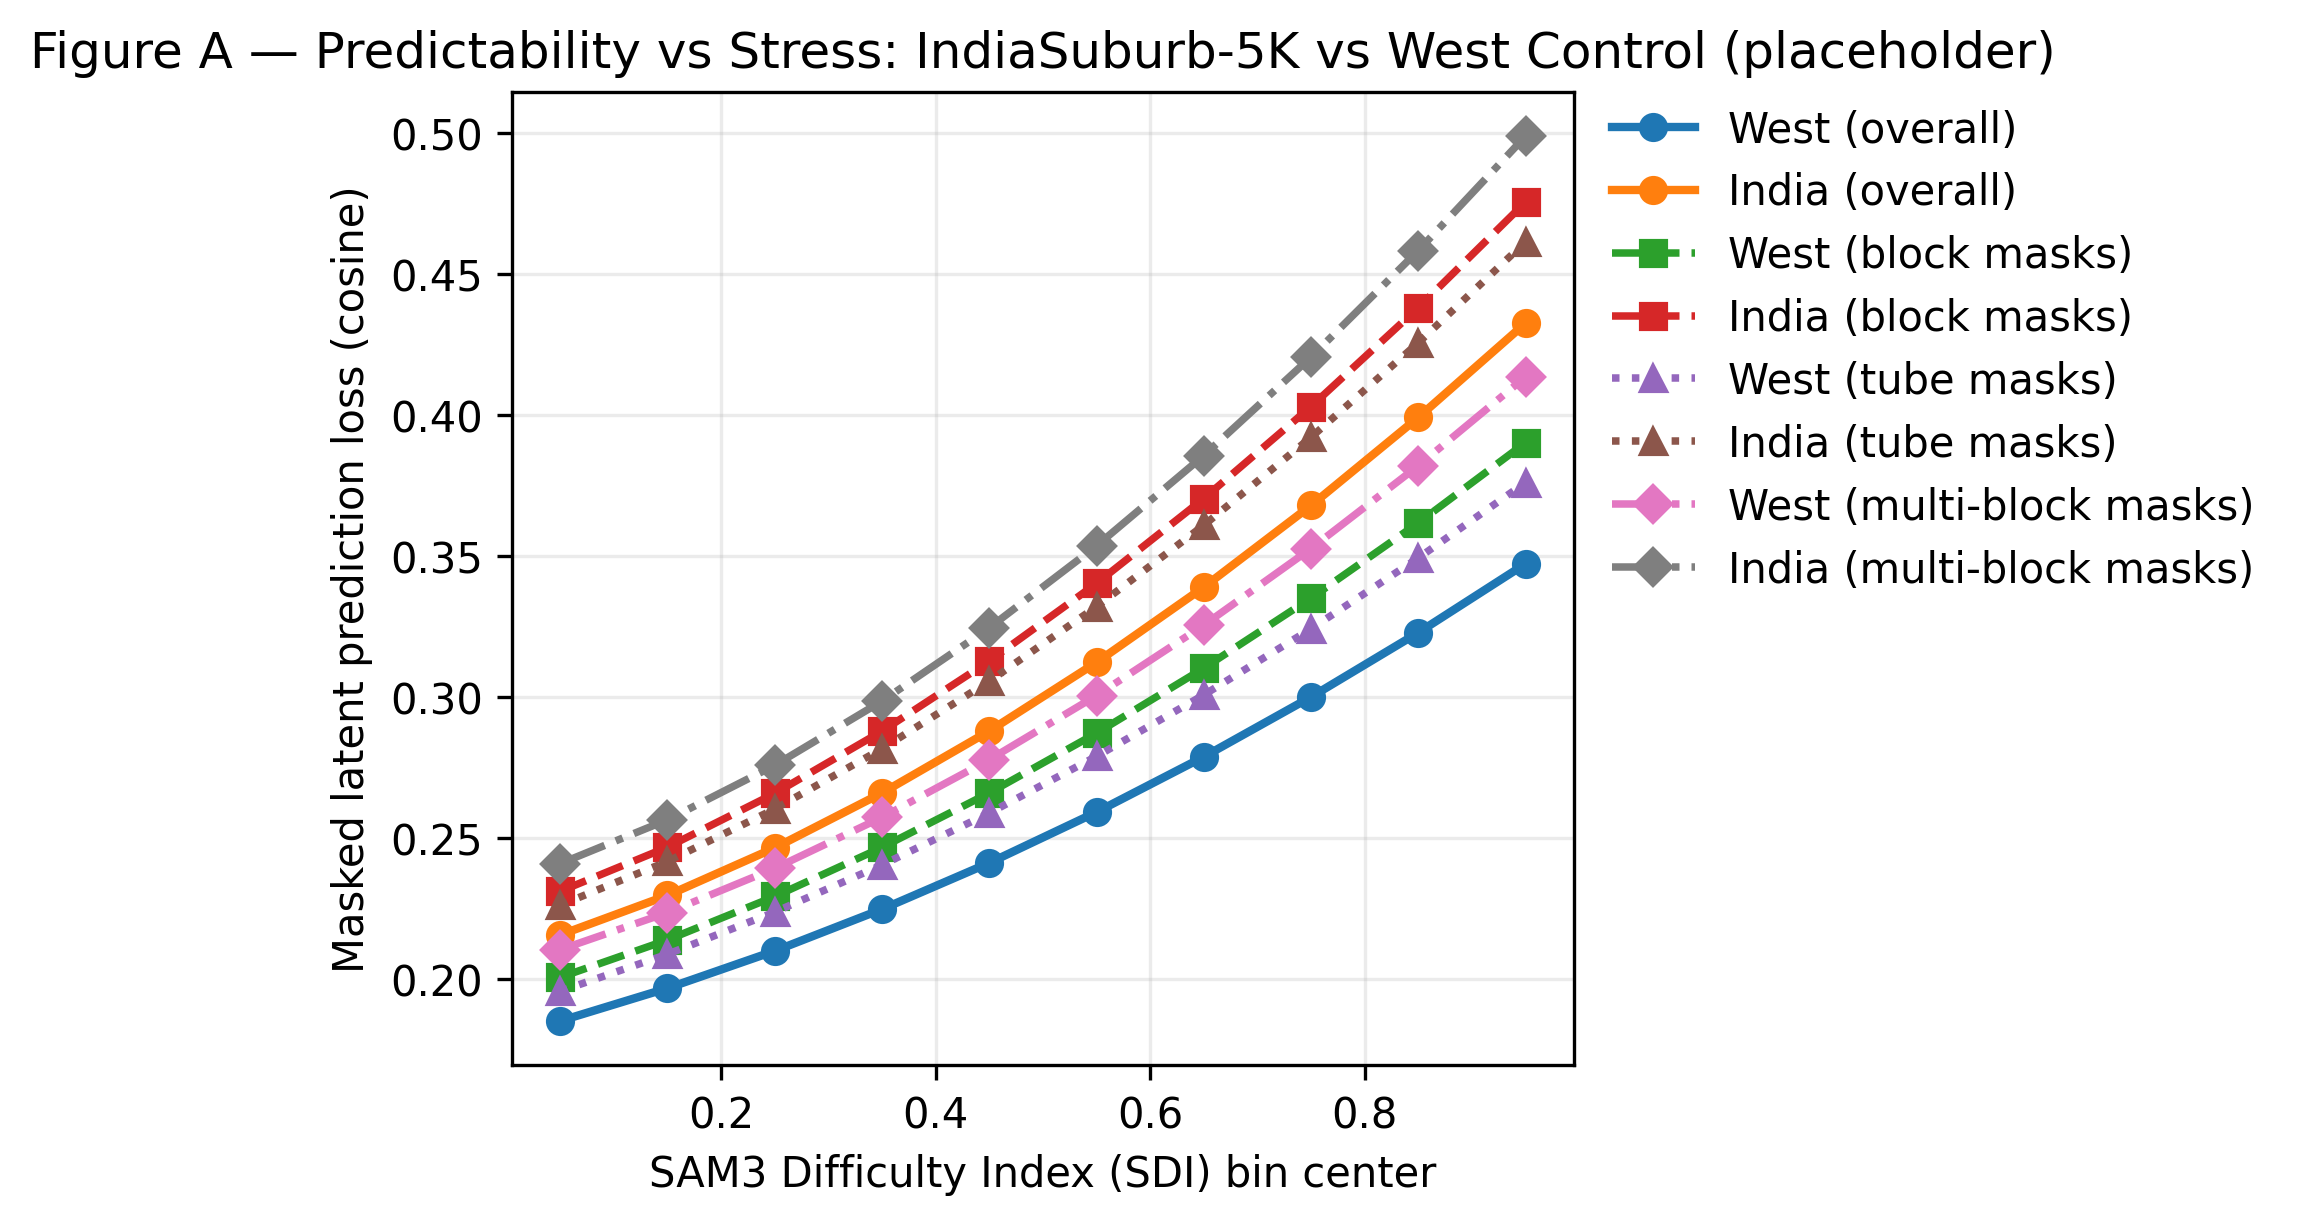
\includegraphics[width=0.95\textwidth]{india/FigA_loss_vs_sdi.png}
  \caption{\textbf{Predictability under Indian street stress: masked-latent prediction loss vs.\ SAM3 Difficulty Index (SDI).}
  We evaluate a frozen V-JEPA 2 checkpoint via masked-latent prediction on \textbf{IndianSuburb-5K} (India) and a matched \textbf{WestSuburb} control set (West), stratifying clips by SDI (x-axis), a deterministic scalar computed from SAM3-only masks/tracklets (density, clutter, occlusion, interaction proximity, and track fragmentation). The y-axis reports the mean masked-latent prediction loss (cosine error in representation space; lower is better), averaged over $K$ random masks per clip and then averaged within each SDI bin; error bars (when shown in the final paper) should be 95\% bootstrap CIs over clips.
  Solid curves show the \textbf{overall} loss, while dashed/dotted curves decompose the objective by \textbf{mask family}: \emph{block} masks emulate contiguous occlusion events, \emph{tube} masks probe motion-consistent trajectories, and \emph{multi-block} masks emulate market-like clutter with multiple separated hidden regions.
  The intended diagnostic signature is a \textbf{stress-amplified domain gap}: as SDI increases (crowding/occlusion/clutter intensify), the India loss curve rises faster than the West curve—especially for block and multi-block masks—indicating that the pretrained predictive mechanism is less calibrated to Indian street ecology where agents frequently overlap, appear/disappear under occlusion, and interact at short spatial margins.}
  \label{fig:exp1_loss_sdi}
\end{figure*}

% -------------------------
% Figure B: Exp-2 (layerwise info-flow)
% -------------------------
\begin{figure*}[t]
  \centering
  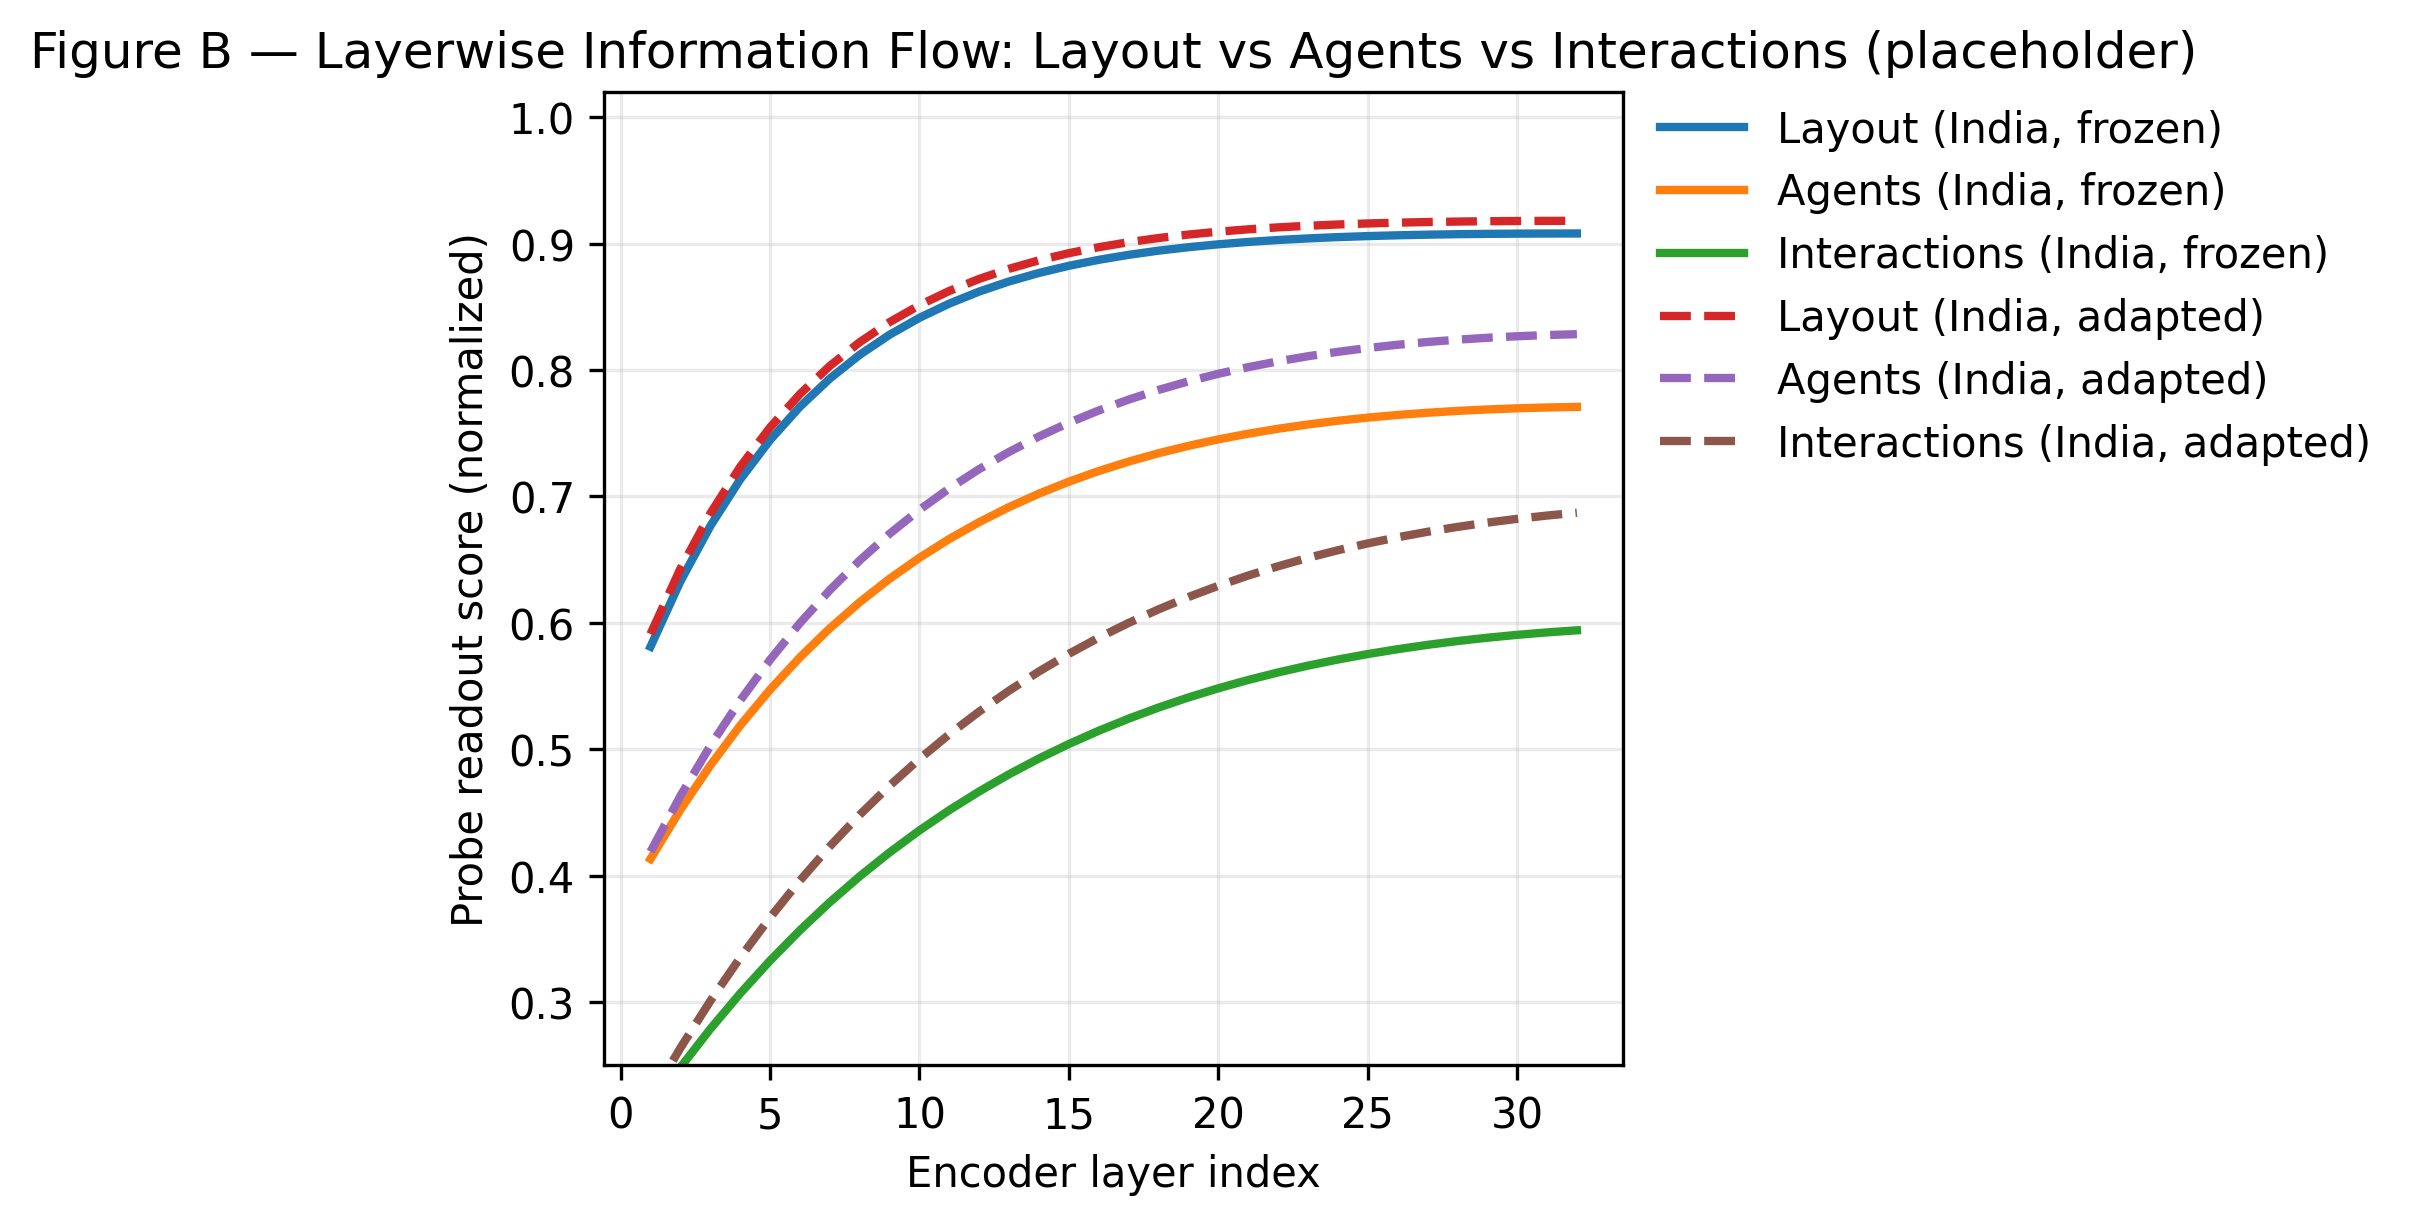
\includegraphics[width=0.95\textwidth]{india/FigB_layerwise_info_flow.png}
  \caption{\textbf{Where is information represented in depth? Layerwise readout for layout, agents, and interactions.}
  Using the V-JEPA 2 encoder as a \textbf{frozen backbone}, we train lightweight probes (linear/attentive probe, identical hyperparameters across domains) to read out three factorized signals from layerwise tokens: \textbf{Layout} (background structure after suppressing SAM3 instances), \textbf{Agents} (instance-centric statistics such as density/heterogeneity derived from SAM3 masks and tracklets), and \textbf{Interactions} (graph/tensor summaries of close-approach events and sustained proximity derived from tracklet geometry).
  The x-axis is the encoder layer index; the y-axis is a normalized probe score (e.g., accuracy/F1 for binned targets or $R^2$ for regression, mapped to a common scale for visualization). Solid curves show readout on IndianSuburb-5K with the \textbf{frozen pretrained} model; dashed curves illustrate the same readouts after \textbf{bounded self-supervised adaptation} on IndianSuburb-5K (e.g., predictor-only, last-$k$ blocks, or adapter tuning; the exact choice should be specified in the caption of the final version).
  The spotlight-ready interpretation is \textbf{factor-specific domain mismatch}: layout is typically accessible earlier and remains comparatively stable, whereas agent and interaction signals require deeper integration and can be substantially degraded by Indian-specific stressors (occlusion, clutter, heterogeneous motion). A right-shifted or depressed interaction curve indicates that the pretrained representation consolidates interaction structure less reliably under the Indian domain and may require additional depth or adaptation to recover robust interaction encoding.}
  \label{fig:exp2_layerwise_flow}
\end{figure*}

% -------------------------
% Figure C: Exp-2 (stress-sliced probing + factor table)
% -------------------------
\begin{figure*}[t]
  \centering
  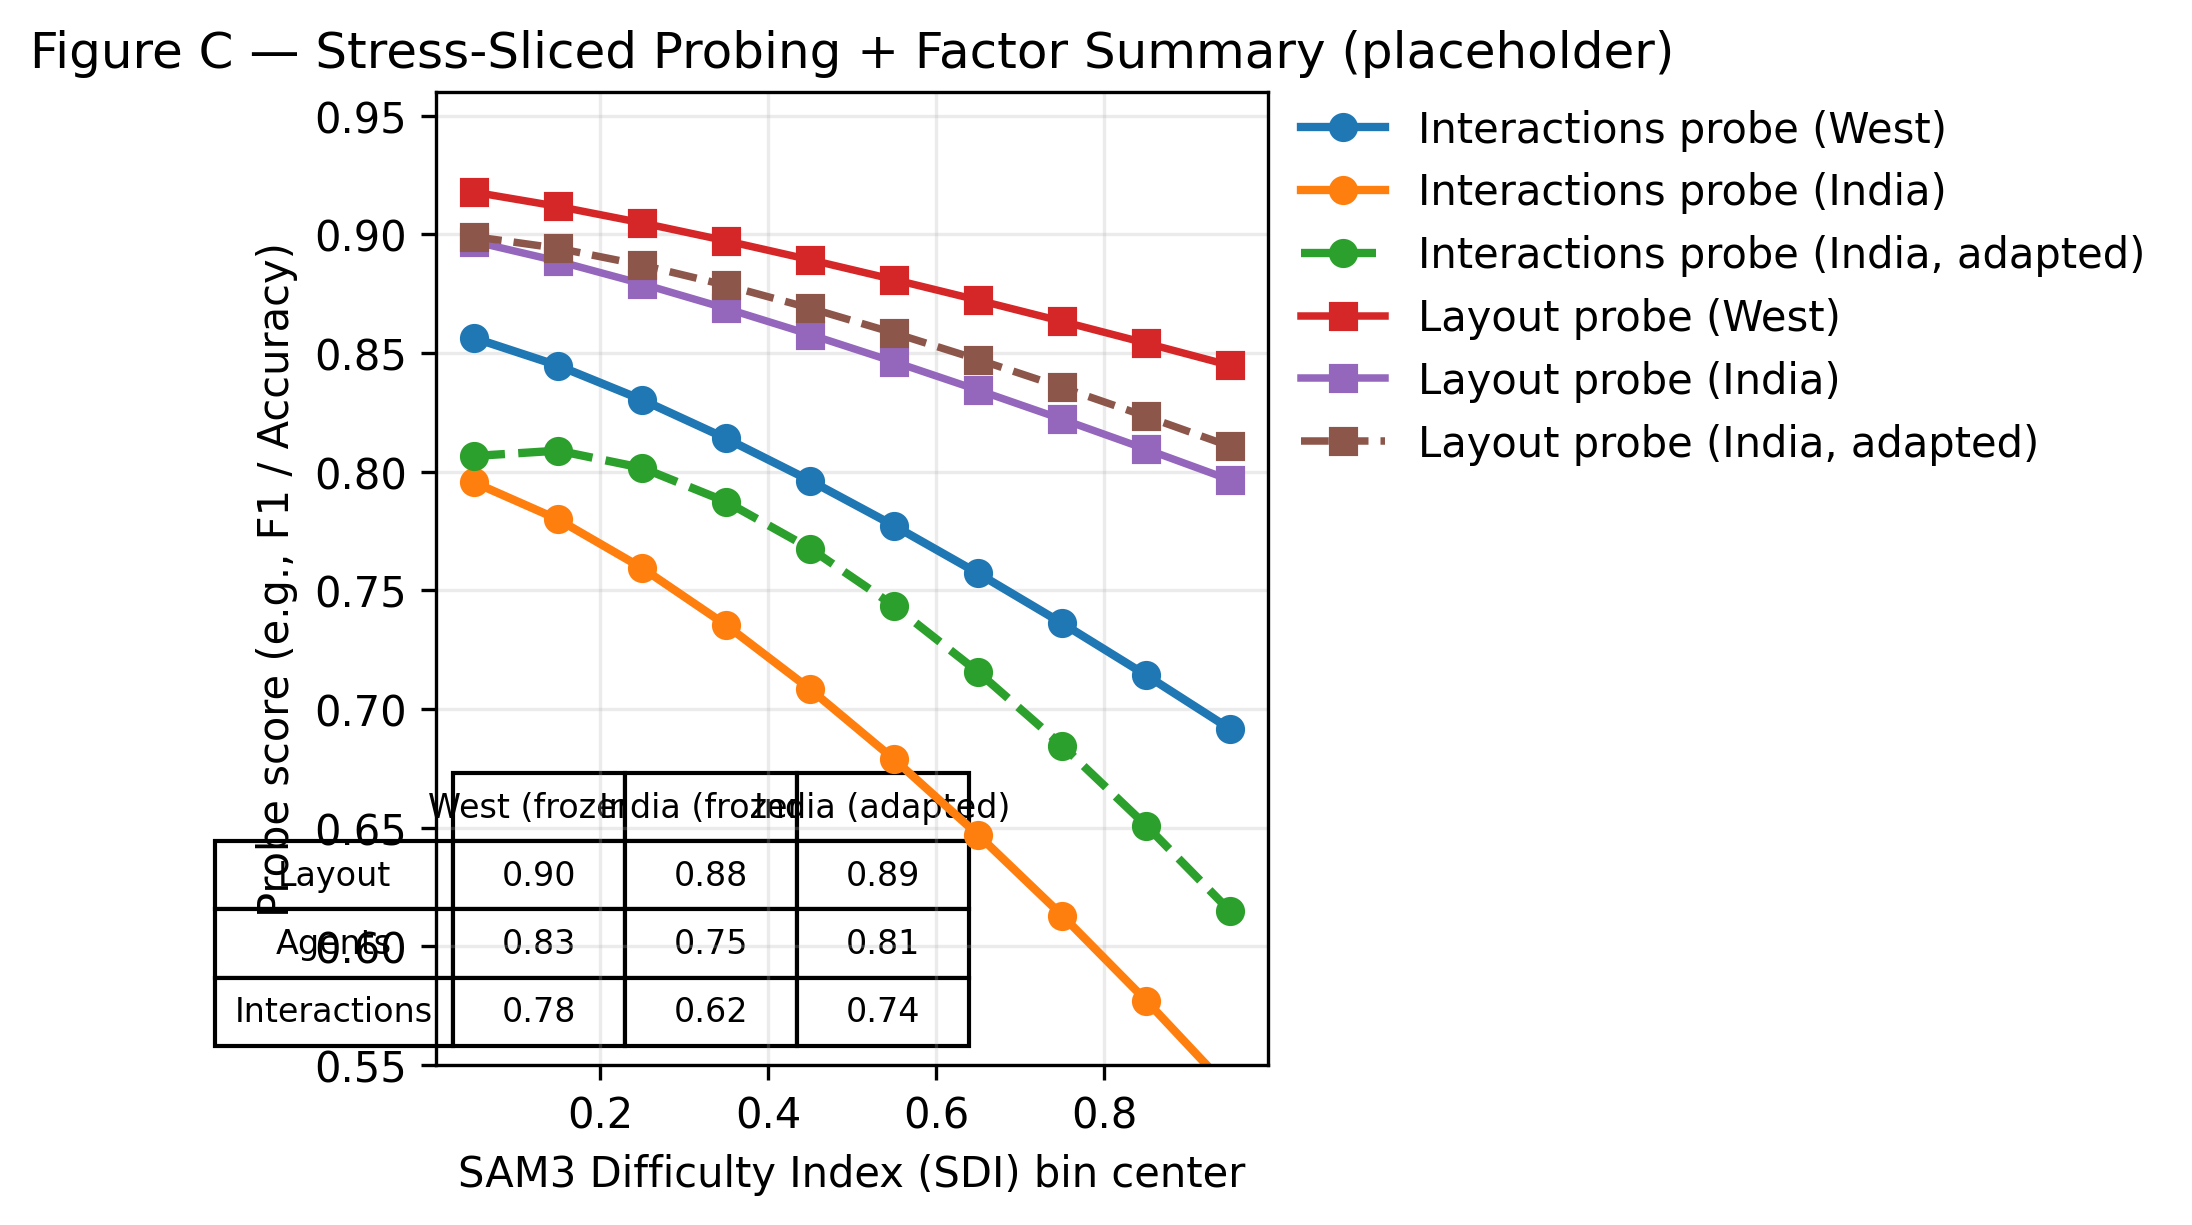
\includegraphics[width=0.95\textwidth]{india/FigC_probe_vs_sdi_with_table.png}
  \caption{\textbf{Stress-sliced probing plus factor summary: interaction readout collapses earlier under Indian stress.}
  We evaluate frozen-backbone probes across SDI bins (x-axis) to measure how readout quality varies with scene stress. Curves depict probe performance (y-axis; e.g., F1/accuracy for binned targets) for \textbf{Interactions} (primary diagnostic) and \textbf{Layout} (stability reference), comparing West control vs IndianSuburb-5K, and optionally an India-adapted variant.
  The embedded factor table summarizes aggregate probe scores over the entire test set for \textbf{Layout}, \textbf{Agents}, and \textbf{Interactions}, enabling a single-glance decomposition of the domain gap: in the expected failure pattern, layout remains near-parity, agents degrade moderately, and interactions degrade most—consistent with Indian suburb streets and markets being dominated by dense, multi-agent negotiation under occlusion and clutter.
  This figure complements Fig.~\ref{fig:exp1_loss_sdi} by localizing \emph{what} predictability loss corresponds to: not just general visual difficulty, but specifically diminished accessibility of interaction structure in latent space as SDI increases.}
  \label{fig:exp2_probe_sdi}
\end{figure*}

% -------------------------
% Figure D: Exp-3 (Pareto tradeoff)
% -------------------------
\begin{figure*}[t]
  \centering
  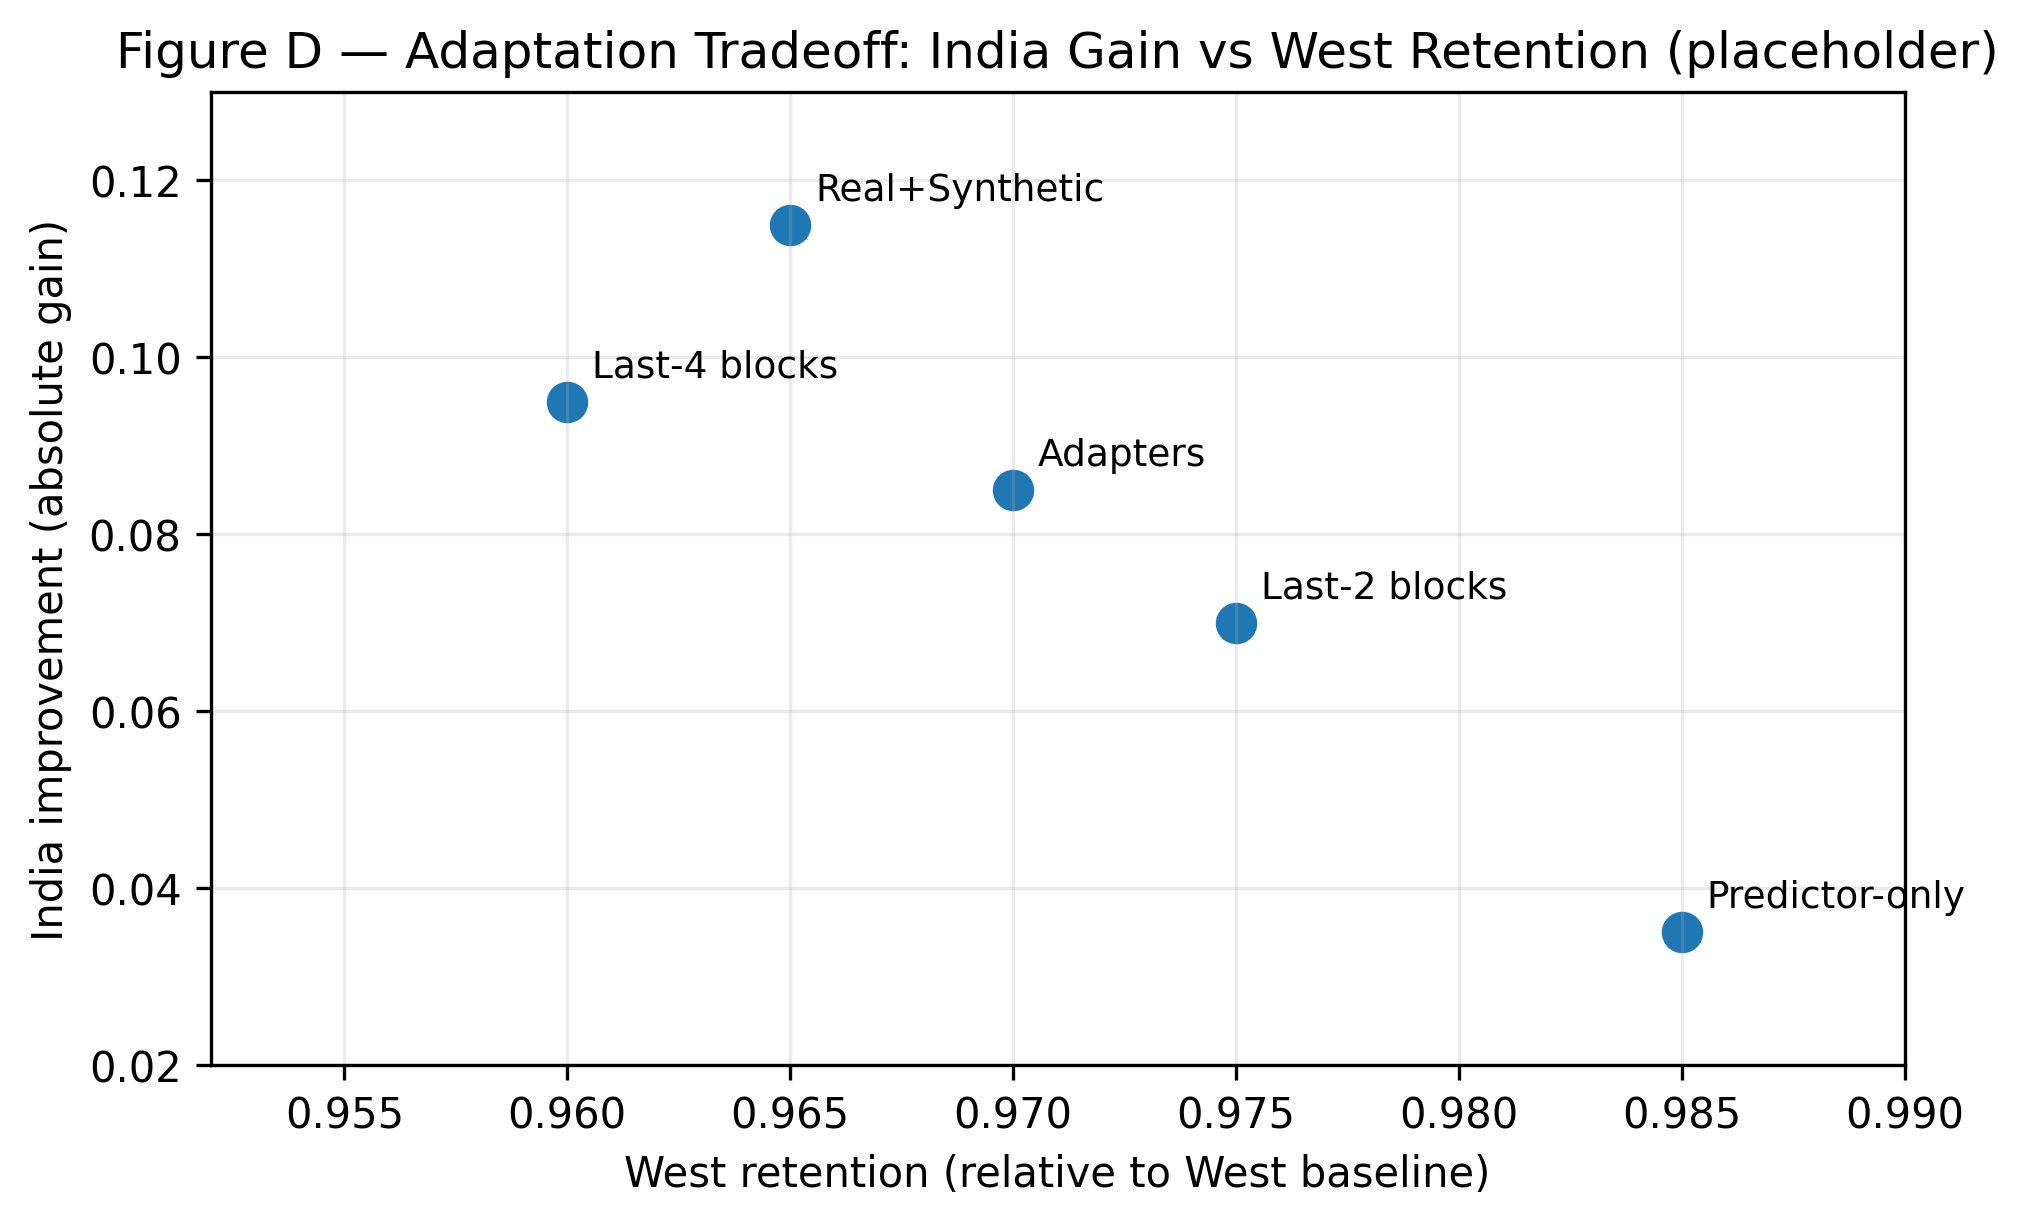
\includegraphics[width=0.95\textwidth]{india/FigD_pareto_tradeoff.png}
  \caption{\textbf{Adaptation tradeoff frontier: India improvement vs West retention.}
  We compare bounded adaptation strategies for mitigating the India domain gap without sacrificing generality. Each point corresponds to a specific adaptation regime (e.g., \emph{predictor-only}, \emph{last-2 blocks}, \emph{last-4 blocks}, \emph{adapters}, and \emph{real+synthetic} adaptation), evaluated after adaptation by re-running Exp-1/Exp-2 metrics on both domains.
  The x-axis measures \textbf{West retention} (performance relative to the original pretrained model on the West control test; higher is better), while the y-axis measures \textbf{India improvement} (absolute gain on IndianSuburb-5K; higher is better). Points nearer the top-right are preferable; a convex frontier indicates a genuine tradeoff between specializing to Indian street ecology and preserving broader generalization.
  This figure is essential for a defensible conclusion: it distinguishes (i) small calibration gains achievable by tuning the predictor alone from (ii) representational gains requiring deeper adaptation, and it quantifies whether adding India-like synthetic videos (generated to stress narrow mixed-traffic roads and dense market occlusion) shifts the frontier upward, i.e., improves India robustness at comparable West retention.}
  \label{fig:exp3_pareto}
\end{figure*}





\subsection{Experiment 1: Predictability Under Indian Dynamics (Masked-Latent Prediction)}
\label{sec:exp1}

\paragraph{What this experiment reveals.}
This is the most “world-model-ish” diagnostic: does a pretrained model find Indian street scenes \emph{predictable in latent space}, or does its predictive mechanism break exactly where India is hard (occlusion, dense interaction, clutter)?

\subsubsection{Exp-1A: Core masked-latent prediction metric}

\paragraph{Masking protocol.}
We run multiple mask patterns per clip to avoid gaming any one pattern:
\begin{itemize}[leftmargin=*,itemsep=2pt]
  \item \textbf{Block masks:} contiguous space-time cuboids (occlusion-like).
  \item \textbf{Tube masks:} track-aligned tubes (motion-like).
  \item \textbf{Multi-block masks:} several separated blocks (market-like clutter).
\end{itemize}
For each clip, sample $K$ masks $\{m_k\}_{k=1}^K$ (e.g., $K{=}8$), with a fixed mask ratio $\rho = |\mathcal{M}|/N$ (e.g., $\rho\in\{0.5,0.75\}$).

\paragraph{Masked-latent prediction loss (unnumbered).}
We measure prediction error in representation space. Two robust choices:
\[
\mathcal{L}_{\cos}(x;m) = \frac{1}{|\mathcal{M}|}\sum_{i\in\mathcal{M}}\left(1 - \frac{\langle \hat{z}_i, z_i \rangle}{\|\hat{z}_i\|\|z_i\|}\right),
\qquad
\mathcal{L}_{\ell_2}(x;m) = \frac{1}{|\mathcal{M}|}\sum_{i\in\mathcal{M}} \|\hat{z}_i - z_i\|_2^2.
\]
We report the per-clip loss averaged over masks:
\[
\overline{\mathcal{L}}(x) = \frac{1}{K}\sum_{k=1}^K \mathcal{L}(x;m_k).
\]

\paragraph{Primary plot (the one that convinces).}
Make SDI the x-axis and masked prediction loss the y-axis:
\begin{itemize}[leftmargin=*,itemsep=2pt]
  \item plot $\mathbb{E}[\overline{\mathcal{L}}(x)\mid \mathrm{SDI}(x)\in \text{bin }b]$ over SDI bins,
  \item show separate curves for \textbf{India} and \textbf{West} under the same bin edges.
\end{itemize}
If West-trained representations internalize “street physics” well, the India curve should track the West curve under matched SDI. If not, India rises faster (predictability collapses earlier).

\subsubsection{Exp-1B: Where does predictability break (mask-type sensitivity)?}

\paragraph{Mask-type decomposition.}
Compute losses per mask family:
\[
\overline{\mathcal{L}}_{\mathrm{block}}(x),\;
\overline{\mathcal{L}}_{\mathrm{tube}}(x),\;
\overline{\mathcal{L}}_{\mathrm{multiblock}}(x).
\]
This lets you localize the failure mode:
\begin{itemize}[leftmargin=*,itemsep=2pt]
  \item \textbf{Occlusion failure:} block/multi-block losses spike in markets.
  \item \textbf{Interaction failure:} tube masks spike when many trajectories cross.
  \item \textbf{Clutter failure:} multi-block spikes when signage clutter is high.
\end{itemize}

\subsubsection{Exp-1C: Token-level error maps (visual evidence, not just curves)}

\paragraph{Token error heatmaps.}
For a sampled clip $x$, compute per-token error
\[
e_i(x;m) = 1 - \frac{\langle \hat{z}_i, z_i \rangle}{\|\hat{z}_i\|\|z_i\|}, \quad i\in\mathcal{M},
\]
and visualize $e_i$ back in space-time (tubelet grid). Overlay (qualitatively) with SAM3 occlusion zones. In Indian markets, you often see “error islands” exactly where humans also struggle: dense overlaps, signboards, stall boundaries, and micro-motions of crowds.

\paragraph{What to report (final Exp-1 metrics).}
\begin{itemize}[leftmargin=*,itemsep=2pt]
  \item mean loss on India vs West (global),
  \item SDI-sliced loss curves (primary),
  \item loss by mask family (diagnostic),
  \item top-1\% hardest clips (qualitative panels + error maps).
\end{itemize}

\subsection{Experiment 2: Factorized Competence (Layout / Agents / Interactions Probing)}
\label{sec:exp2}

\paragraph{What this experiment reveals.}
Exp-1 says “predictability changed.” Exp-2 says \emph{what information is missing} in the representation: geometry, agents, or interaction structure. This directly connects to your FactorJEPA framing.

\subsubsection{Exp-2A: Factorized views and derived targets}

\paragraph{Three factor streams.}
From the same clip $x$, create:
\begin{itemize}[leftmargin=*,itemsep=2pt]
  \item \textbf{Layout view} $x^{(L)}$: background-only (agents removed by SAM3 masks).
  \item \textbf{Agents view} $x^{(A)}$: agents-only (everything outside masks suppressed).
  \item \textbf{Interaction tensor} $x^{(I)}$: track-graph summary (pairwise proximity over time).
\end{itemize}

\paragraph{Targets without manual labels.}
We deliberately choose targets that come “for free” from SAM3 + tracking and are still meaningful:
\begin{itemize}[leftmargin=*,itemsep=2pt]
  \item \textbf{Layout targets:} clutter percentile class, static-structure complexity (edge density / entropy), camera motion regime (low/medium/high).
  \item \textbf{Agent targets:} density class, heterogeneity class (size/speed/aspect entropy), mean speed bins, track fragmentation bins.
  \item \textbf{Interaction targets:} interaction-count bins, near-contact event presence, sustained crowding (duration above proximity threshold).
\end{itemize}
All targets are defined by percentile thresholds computed on the training split and held fixed.

\subsubsection{Exp-2B: Frozen attentive probe protocol (V-JEPA 2 style)}

\paragraph{Backbone frozen, probe trained.}
We freeze $f_{\theta}$ and train a small attentive probe $h_{\psi}$ on top of selected layers’ tokens. The V-JEPA 2 paper describes a 4-layer attentive probe with a final cross-attention layer using learnable query token(s); we follow the same spirit. :contentReference[oaicite:0]{index=0}

\paragraph{Multi-layer token input (important).}
For each selected encoder layer set $\mathcal{S}=\{\ell_1,\dots,\ell_r\}$, collect tokens
\[
u = \mathrm{concat}\big(z^{(\ell_1)},\dots,z^{(\ell_r)}\big),
\]
and feed to the probe. This captures the known phenomenon that some tasks (especially motion/interaction) benefit from deeper tokens plus mid-layer structure.

\paragraph{Probe losses.}
For classification tasks (bin labels) use cross-entropy:
\[
\mathcal{L}_{\mathrm{CE}} = -\sum_{c} y_c \log p_{\psi}(c\mid u),
\]
and for scalar regression tasks (e.g., density) use Huber or $\ell_2$:
\[
\mathcal{L}_{\mathrm{reg}} = \| \hat{y} - y\|_2^2 \quad \text{or} \quad \mathrm{Huber}(\hat{y}-y).
\]

\paragraph{Factor probes as a matrix (the core table).}
Train probes for each factor stream and evaluate on India test:
\begin{itemize}[leftmargin=*,itemsep=2pt]
  \item Layout-probes on $x^{(L)}$,
  \item Agent-probes on $x^{(A)}$,
  \item Interaction-probes on $x^{(I)}$ (via tokens from $x$ or via a small MLP on interaction tensor).
\end{itemize}
Report a compact grid of metrics: accuracy/F1 for bin tasks, $R^2$ for regression.

\subsubsection{Exp-2C: “Where in depth is India information represented?”}

\paragraph{Layerwise information-flow curves.}
For a fixed probe family, vary which layer tokens are accessible:
\[
\mathcal{S}\in \{\{\ell\}\;|\;\ell=1,\dots,L\},
\quad \text{or}\quad
\mathcal{S}=\{\ell-3,\ell-2,\ell-1,\ell\}.
\]
Plot probe performance vs layer index. Do this separately for layout / agents / interactions. The resulting “three-channel depth plot” is exactly your desired visualization: x-axis = layer, y-axis = information readout.

\paragraph{Interpretation.}
In many video encoders, static cues stabilize earlier, while interaction cues consolidate later. IndianSuburb often shifts this: heavy occlusion and clutter can delay clean agent encoding; interaction signatures become noisier and require deeper aggregation. This is measurable as:
\begin{itemize}[leftmargin=*,itemsep=2pt]
  \item a right-shift of peak interaction readout,
  \item a widening of the layer band needed to achieve stable performance,
  \item increased sensitivity to multi-layer token input.
\end{itemize}

\subsubsection{Exp-2D: Stress-sliced probing (the second convincing plot)}

\paragraph{Probe performance vs SDI.}
For each probe, compute performance in SDI bins:
\[
\mathrm{Perf}(b) = \mathbb{E}\big[\mathrm{metric}(x)\mid \mathrm{SDI}(x)\in b\big].
\]
Plot $\mathrm{Perf}(b)$ for India and West. When you see a sharp India-only collapse in interaction-probes as SDI increases, you have a crisp narrative: the representation does not retain interaction structure under India-specific congestion.

\paragraph{What to report (final Exp-2 metrics).}
\begin{itemize}[leftmargin=*,itemsep=2pt]
  \item factor-grid probe table (layout/agents/interactions),
  \item layerwise information-flow plots (three-channel),
  \item SDI-sliced probe curves (India vs West),
  \item a small qualitative panel: clips where probes fail, with SAM3 overlays.
\end{itemize}

\subsection{Experiment 3: Domain Gap + Minimal Adaptation Reality-Check}
\label{sec:exp3}

\paragraph{What this experiment reveals.}
Exp-3 answers the question a reviewer will immediately ask: if pretrained V-JEPA 2 struggles, is the fix “just train a bit on India”? We quantify the gap and how much minimal, non-labeled adaptation closes it.

\subsubsection{Exp-3A: Domain Gap Score (DGS) under matched stress}

\paragraph{Matched SDI bins across domains.}
Compute SDI using the same definition on India and West. Define shared bin edges from the union distribution.

\paragraph{Gap metric.}
For any metric $M$ (masked prediction loss, probe accuracy, etc.), define:
\[
\mathrm{DGS}_M(b) = 
\begin{cases}
M_{\mathrm{West}}(b) - M_{\mathrm{India}}(b) & \text{if higher is better (accuracy/F1)}\\
M_{\mathrm{India}}(b) - M_{\mathrm{West}}(b) & \text{if lower is better (loss)}
\end{cases}
\]
and report DGS across bins and its area-under-curve:
\[
\mathrm{DGS\text{-}AUC}_M = \sum_{b} w_b \,\mathrm{DGS}_M(b),
\quad w_b = \frac{|b|}{\sum_{b'} |b'|}.
\]
This collapses “how bad is the India gap” into one scalar per evaluation axis.

\subsubsection{Exp-3B: Minimal self-supervised adaptation (no labels, no semantics)}

\paragraph{Adaptation protocol.}
We do a limited, controlled adaptation on IndianSuburb-5K train clips using the same masked-latent objective, but in a strictly bounded way:
\begin{itemize}[leftmargin=*,itemsep=2pt]
  \item \textbf{Option 1 (light):} freeze encoder $f_{\theta}$, finetune only predictor $g_{\phi}$ for $E$ epochs.
  \item \textbf{Option 2 (moderate):} finetune last $k$ encoder blocks + predictor (e.g., $k\in\{2,4\}$), keep earlier blocks frozen.
  \item \textbf{Option 3 (adapter):} insert small adapters in selected blocks, train adapters + predictor only.
\end{itemize}
All three keep the “foundation” intact and isolate whether India requires representational rewiring or just predictive recalibration.

\paragraph{Why these choices are scientifically clean.}
They let you attribute improvements:
\begin{itemize}[leftmargin=*,itemsep=2pt]
  \item predictor-only gains $\Rightarrow$ latent dynamics mismatch (planning/prediction calibration),
  \item last-block gains $\Rightarrow$ high-level aggregation mismatch (interaction consolidation),
  \item adapter gains $\Rightarrow$ localized representational gap without full retraining.
\end{itemize}

\paragraph{Evaluation after adaptation.}
Re-run Exp-1 and Exp-2 frozen evaluations on India test and West test:
\begin{itemize}[leftmargin=*,itemsep=2pt]
  \item if adaptation helps India but hurts West, you expose specialization,
  \item if adaptation helps both, you likely learned general crowd/occlusion robustness.
\end{itemize}

\subsubsection{Exp-3C: Synthetic augmentation lever (YouTube-only vs YouTube+Sora-style)}

\paragraph{Two training mixtures.}
Using your plan to generate India-like synthetic videos (Sora / Firefly / etc.), define:
\begin{itemize}[leftmargin=*,itemsep=2pt]
  \item \textbf{Real-only:} adaptation on IndianSuburb-5K train clips.
  \item \textbf{Real+Synthetic:} adaptation on IndianSuburb-5K plus synthetic clips targeting narrow roads, dense markets, signage clutter, animals.
\end{itemize}
Run the same bounded adaptation (predictor-only / last-$k$ / adapters) and compare DGS reductions. This isolates whether synthetic data acts as an effective “stress amplifier” for interaction and occlusion.

\paragraph{Key plots for Exp-3.}
\begin{itemize}[leftmargin=*,itemsep=2pt]
  \item DGS vs SDI bins (before/after adaptation),
  \item delta-improvement curves: $\Delta M(b)=M_{\text{adapted}}(b)-M_{\text{base}}(b)$,
  \item a Pareto plot: India gain vs West retention.
\end{itemize}

\subsection{Measurement, Statistics, and Reporting (Make It Reviewer-Proof)}
\label{sec:measurement}

\paragraph{Bootstrapped confidence intervals (clip-level).}
For any reported scalar metric $\hat{\mu}$ (mean loss, mean accuracy), compute 95\% bootstrap CI by resampling clips:
\[
\{\hat{\mu}^{(b)}\}_{b=1}^{B}, \quad \mathrm{CI}_{95} = [\mathrm{pct}_{2.5}(\hat{\mu}^{(b)}), \mathrm{pct}_{97.5}(\hat{\mu}^{(b)})],
\]
with $B$ large enough (e.g., 2000). This is essential when bins are smaller (high SDI tail).

\paragraph{Paired testing where possible.}
If you build matched pairs (India clip vs West clip with similar SDI, motion, camera type), use paired differences to reduce variance:
\[
\Delta(x_i) = M(x_i^{\mathrm{India}}) - M(x_i^{\mathrm{West}}),
\quad \text{report } \mathbb{E}[\Delta] \text{ and its CI}.
\]

\paragraph{Confound controls (do not skip).}
For every “India is worse” claim, also report the same metric under:
\begin{itemize}[leftmargin=*,itemsep=2pt]
  \item camera-type matched subset (dashcam-only, handheld-only),
  \item day-only subset,
  \item motion-matched bins (similar motion intensity).
\end{itemize}
This prevents reviewers from attributing the gap to cinematography rather than scene ecology.

\subsection{Execution Plan (Concrete, End-to-End)}
\label{sec:execution_plan}

\paragraph{Step 1: Prepare data in V-JEPA 2 format.}
Convert IndianSuburb-5K clips into a directory + manifest format compatible with the V-JEPA 2 repo dataset loaders (or implement a minimal dataset class under \texttt{src/datasets/}). The unit must yield clips as tensors plus metadata (clip\_id, SDI, pillar).

\paragraph{Step 2: Download pretrained V-JEPA 2 checkpoints.}
Use official checkpoints (e.g., ViT-L/H/g at 256 or ViT-g at 384) from the repository’s links. :contentReference[oaicite:1]{index=1}

\paragraph{Step 3: Run Exp-1 inference (masked prediction).}
Freeze encoder + predictor; compute $\overline{\mathcal{L}}(x)$ for each clip and each mask family; write \texttt{pred\_loss.csv} with columns:
\[
(\texttt{clip\_id}, \texttt{domain}, \texttt{pillar}, \texttt{SDI}, \mathcal{L}_{\cos}, \mathcal{L}_{\ell_2}, \mathcal{L}_{\mathrm{block}}, \mathcal{L}_{\mathrm{tube}}, \mathcal{L}_{\mathrm{multiblock}}).
\]

\paragraph{Step 4: Train attentive probes (Exp-2).}
Freeze encoder; train probe heads for each factor task. Keep hyperparameters fixed across India and West to ensure comparability. Follow the repo’s evaluation structure (attentive probe training on frozen features). 

\paragraph{Step 5: Build the three flagship figures.}
\begin{itemize}[leftmargin=*,itemsep=2pt]
  \item \textbf{Fig-A (Exp-1):} SDI-sliced masked prediction loss (India vs West; mask families).
  \item \textbf{Fig-B (Exp-2):} three-channel layerwise information-flow curves (layout/agents/interactions).
  \item \textbf{Fig-C (Exp-3):} DGS vs SDI before/after adaptation (Real-only vs Real+Synthetic).
\end{itemize}

\paragraph{Step 6: Adaptation (Exp-3) and re-evaluate.}
Run bounded adaptation options (predictor-only / last-$k$ / adapters), then rerun Exp-1 and Exp-2 on frozen evaluation. Report trade-offs (India gain vs West retention).

\subsection{Expected Outcomes (What “Mostly Ineffective” Looks Like Quantitatively)}
\label{sec:expected_outcomes}

\paragraph{A strong failure pattern.}
You can credibly argue “ineffective” if you observe a consistent triad:
\begin{itemize}[leftmargin=*,itemsep=2pt]
  \item \textbf{Predictability collapse:} India masked prediction loss rises sharply in the high-SDI tail relative to West, especially for block/multi-block masks (occlusion + clutter).
  \item \textbf{Interaction probe fragility:} interaction readout degrades earlier in depth and falls faster with SDI on India, even when layout readout remains stable.
  \item \textbf{Gap persistence after light adaptation:} predictor-only adaptation helps slightly, but the SDI-tail gap remains large unless deeper blocks/adapters adapt, indicating representational mismatch rather than mere calibration.
\end{itemize}

\paragraph{A clean “what fixes it” story.}
If Real+Synthetic reduces DGS more than Real-only in interaction-heavy bins, you get a compelling narrative: targeted synthetic stressors can efficiently teach the missing Indian interaction priors, even without semantic labels.

\paragraph{Deliverable.}
At the end of these three experiments, you have a complete spotlight-ready evaluation: one dataset, one backbone, three complementary lenses (predictability, factorized competence, domain-gap adaptation), and figures that make the India-specific difficulty not anecdotal but \textbf{measured, sliced, and reproducible}.































\section{Factorizing V-JEPA2 for India Adoption (Practical, K-FAC Aware)}
\label{sec:factorize_vjepa2_india_practical_kfac}

\paragraph{Positioning (why this section exists).}
We assume a realistic academic constraint: \textbf{we cannot pretrain V-JEPA2 from scratch}. Our goal is therefore operational and auditable: \textbf{start from a released V-JEPA2 checkpoint} and adapt it to India using \textbf{Option-C updates only} (LoRA/adapters in the last $k$ blocks, optionally the predictor), while making the failure modes \emph{measurable} via factor channels. This section is implementation-first: it specifies \textbf{(i) what code paths we modify}, \textbf{(ii) what we train and freeze}, \textbf{(iii) what statistics we cache}, \textbf{(iv) what optimizers we run}, and \textbf{(v) what we log and plot}. We do \emph{not} re-describe dataset collection; we assume IndianSuburb-5K is already prepared and SAM3 caches are available from the earlier pipeline.

\vspace{4pt}
\paragraph{Two principles we enforce throughout.}
\begin{itemize}[leftmargin=*,itemsep=2pt]
\item \textbf{Channels are not created by LoRA.} Layout/Agents/Interactions channels are created by \textbf{factor views + SAM3-derived targets + probes/heads}. LoRA/adapters only provide a low-budget way for the checkpoint to change.
\item \textbf{Optimizer comparisons must be fair.} AdamW, Shampoo, and K-FAC-Lite all see the \textbf{same trainable parameters}, \textbf{same loss}, and \textbf{same budget}. Any difference is therefore due to update geometry, not different degrees of freedom.
\end{itemize}

\subsection{Frozen truth: checkpoint locking and reproducibility contract}
\label{sec:checkpoint_locking_contract}

\paragraph{Lock the base checkpoint.}
We define a base checkpoint $C_0$ by \textbf{(identifier, repository commit, weight hash)}. This triple is immutable during the project. All adaptations are stored as \textbf{delta artifacts} (LoRA/adapter weights and optional predictor deltas) with their own hashes. Students should be able to recover $C_0$ at any time by disabling deltas.

\paragraph{Reproducibility metadata (must be logged).}
Each run logs:
\begin{itemize}[leftmargin=*,itemsep=2pt]
\item model: checkpoint id, commit hash, weight SHA,
\item input: fps, resolution, clip length $T$, masking family mix,
\item adaptation: $k$ (last-$k$ blocks), LoRA rank $r$ or adapter bottleneck $r$, optimizer choice, schedule,
\item evaluation: SDI bin thresholds and the exact India/West split identifiers.
\end{itemize}

\subsection{Where IndianSuburb-5K enters the system (three roles, compact)}
\label{sec:india_roles_compact}

We use IndianSuburb-5K in three roles; we keep them distinct to avoid interpretability confusion.

\paragraph{Role I: adaptation distribution.}
Clips from IndianSuburb-5K provide the self-supervised training distribution for bounded adaptation. The JEPA masked prediction loss is optimized on these clips.

\paragraph{Role II: factor scaffolding via cached SAM3 outputs.}
Cached SAM3 masks and tracklets provide deterministic factor views and factor targets (layout/agents/interactions), plus SDI and visibility gating statistics.

\paragraph{Role III: stress-stratified evaluation.}
We evaluate on India test clips (and a West-matched control set) stratified by SDI bins to measure where failures concentrate (typically high SDI).

\subsection{Option-C adaptation: what changes, where it changes (no ambiguity)}
\label{sec:option_c_what_changes}

\paragraph{Adaptation region: last $k$ blocks.}
Let the encoder be a stack of $L$ transformer blocks. We adapt only the last $k$ blocks (default $k=2$, ablate $k=4$) and freeze all earlier blocks. This makes adaptation compute-feasible and isolates changes to late integration.

\paragraph{LoRA update rule (effective weight view).}
For any Linear map with weight $W\in\mathbb{R}^{o\times i}$ in the last $k$ blocks (attention/MLP projections), we freeze $W$ and learn a low-rank residual:
\[
W' \;=\; W + \Delta W,
\qquad
\Delta W \;=\; \alpha\, B A,
\]
where $A\in\mathbb{R}^{r\times i}$ and $B\in\mathbb{R}^{o\times r}$ are trainable, $r\ll\min(o,i)$, and $\alpha$ is a scale. The base checkpoint remains intact; only $(A,B)$ are learned.

\paragraph{Adapter alternative (same adaptation region).}
Instead of LoRA, we may insert a bottleneck residual adapter in the last $k$ blocks:
\[
h' \;=\; h + U\,\sigma(Vh),
\]
with $V\in\mathbb{R}^{r\times d}$ and $U\in\mathbb{R}^{d\times r}$ trainable. The remainder of the checkpoint is frozen.

\paragraph{Predictor tuning (optional, but held fixed across optimizer comparisons).}
If we unfreeze the predictor head, we do it for \emph{all} optimizers in the comparison. Otherwise, it remains frozen for all. We do not mix predictor-on and predictor-off within the optimizer study.

\subsection{Channel factorization is enforced by views/targets, not by LoRA}
\label{sec:factor_channels_enforced}

\paragraph{Factor views (computed deterministically from cached SAM3 masks).}
Using cached masks/tracklets, we define:
\begin{itemize}[leftmargin=*,itemsep=2pt]
\item \textbf{Layout view} $x^{(L)}$: suppress instance pixels, keep background.
\item \textbf{Agents view} $x^{(A)}$: keep instance pixels, suppress background.
\item \textbf{Interaction summary} $x^{(I)}$: a graph/tensor derived from tracklets (proximity, crossing, merging, occlusion events).
\end{itemize}
These views are what make ``three channels'' concrete and executable.

\paragraph{Visibility/occlusion gate.}
We compute a scalar gate $\gamma(x)\in[0,1]$ from cached SAM3 statistics (occlusion, fragmentation, density). This implements our preferred framing: \textbf{FactorJEPA = 3 factors + 1 visibility gate}, and it is used only to reweight auxiliary terms and stress reporting.

\paragraph{Two minimal ways to realize channels in training/evaluation (we support both).}
\begin{itemize}[leftmargin=*,itemsep=2pt]
\item \textbf{Probes-only (simplest).} Train adaptation with the JEPA loss only; quantify factor channels via layerwise probes predicting factor targets. This keeps training closest to the released objective.
\item \textbf{Factor-guided (recommended).} Add three tiny heads $h_L,h_A,h_I$ trained on SAM3-derived targets to shape gradients toward interaction robustness under India stress. This does not require human labels and keeps trainable capacity dominated by LoRA/adapters.
\end{itemize}

\subsection{Training loss (JEPA + optional factor guidance, identical across optimizers)}
\label{sec:training_loss_kfac_section}

\paragraph{Main loss: masked latent prediction.}
For each clip $x$, sample $K$ masks (block / multi-block / tube). Let $\mathcal{M}_k$ be masked token indices for mask $k$; the predictor produces $\hat{z}_{\mathcal{M}_k}$ from visible context. We optimize:
\[
\mathcal{L}_{\text{pred}}(x) \;=\; \frac{1}{K}\sum_{k=1}^{K}\frac{1}{|\mathcal{M}_k|}\sum_{i\in\mathcal{M}_k}
\Big(1 - \frac{\langle \hat{z}_i, z_i\rangle}{\|\hat{z}_i\|\|z_i\|}\Big).
\]
Masking families are mixed to reflect India-like occlusion and motion.

\paragraph{Optional factor-guided auxiliary (small heads, SAM3-only).}
We define deterministic targets $y_L,y_A,y_I$ from cached SAM3 signals and train small heads:
\[
\mathcal{L}_{\text{factor}}(x)
=
\lambda_L(\gamma)\,\mathcal{L}_L(h_L(f(x^{(L)})),y_L)
+
\lambda_A(\gamma)\,\mathcal{L}_A(h_A(f(x^{(A)})),y_A)
+
\lambda_I(\gamma)\,\mathcal{L}_I(h_I(f(x),x^{(I)}),y_I),
\]
where $\lambda_\cdot(\gamma)$ are simple gate-weighted scalars (increase interaction emphasis when visibility is low). Heads are small (linear or 2-layer MLP); LoRA/adapters remain the main trainable capacity.

\paragraph{Total loss.}
\[
\mathcal{L}_{\text{adapt}}(x)
\;=\;
\mathcal{L}_{\text{pred}}(x)
+
\mathcal{L}_{\text{factor}}(x)
\qquad
(\text{or } \mathcal{L}_{\text{factor}} \equiv 0 \text{ for probes-only}).
\]
This total loss is held fixed across all optimizer runs.

\subsection{Optimizer study (fair, practical, and K-FAC aware)}
\label{sec:optimizer_study_kfac}

We compare three optimizers for Option-C adaptation under \textbf{identical trainable parameters, loss, and budget}:
\begin{itemize}[leftmargin=*,itemsep=2pt]
\item \textbf{AdamW} (baseline),
\item \textbf{Shampoo} (practical structured preconditioning for matrix parameters),
\item \textbf{K-FAC-Lite} (hook-based Kronecker preconditioning applied only to adapted layers, with robust fallback).
\end{itemize}
All three optimize only the LoRA/adapter parameters (and optionally the predictor, if enabled for all).

\subsubsection{AdamW (baseline)}
\label{sec:adamw_plan}

\paragraph{What it updates.}
AdamW updates only LoRA/adapter parameters; base checkpoint weights are frozen. If the predictor is unfrozen, it is placed in a separate parameter group (often with a smaller learning rate).

\paragraph{Practical defaults (students can run today).}
We use warmup + cosine decay, gradient clipping, and mixed precision if available. We log per-step time, gradient norms, and evaluation metrics at fixed intervals. AdamW serves as the reference for stability and compute cost.

\subsubsection{Shampoo (recommended practical second-order-ish baseline)}
\label{sec:shampoo_plan}

\paragraph{Where Shampoo applies.}
Shampoo is applied only to matrix-shaped LoRA/adapter parameters $(A,B)$ or $(U,V)$. Any scalar/bias parameters (if present) remain on Adam-style updates. This avoids pathological behavior on tiny parameters.

\paragraph{Key implementation knobs.}
We use block partitioning for large matrices, infrequent inverse-root updates, and (if available) grafting to Adam-style step magnitudes. The expected outcomes we test are:
\begin{itemize}[leftmargin=*,itemsep=2pt]
\item fewer unstable steps in high-SDI training segments,
\item faster improvement at fixed step budget,
\item better India-vs-West Pareto points.
\end{itemize}

\subsubsection{K-FAC-Lite (LoRA-compatible, hook-based, failure-safe)}
\label{sec:kfac_lite_plan}

\paragraph{Scope (so it is implementable).}
We apply K-FAC-Lite only to Linear layers in the last $k$ blocks that are adapted (start with MLP projections; optionally include attention projections after stability is confirmed). We do not attempt full-model K-FAC.

\paragraph{What statistics K-FAC-Lite needs (derivatives in practice).}
For each adapted Linear layer $y = W x$ we collect:
\begin{itemize}[leftmargin=*,itemsep=2pt]
\item \textbf{Activation samples} $x$ from the forward pass,
\item \textbf{Output-gradient samples} $g=\partial \mathcal{L}/\partial y$ from the backward pass.
\end{itemize}
To keep runtime feasible, we compute covariances on a \textbf{token-subsampled} set of activations/gradients per step (random subset of tokens across batch and time).

\paragraph{Kronecker factors (EMA).}
We maintain exponential moving averages:
\[
A \leftarrow \rho A + (1-\rho)\,\widehat{A},\qquad
\widehat{A} = \mathbb{E}[x x^\top],
\]
\[
G \leftarrow \rho G + (1-\rho)\,\widehat{G},\qquad
\widehat{G} = \mathbb{E}[g g^\top],
\]
with $\rho$ chosen for stability. We apply damping:
\[
A_d = A + \lambda I,\qquad G_d = G + \lambda I,
\]
and update Cholesky factors of $A_d$ and $G_d$ only every $M$ steps (infrequent inversion).

\paragraph{Preconditioning in weight-space (the LoRA bridge).}
K-FAC is defined in the space of weight gradients. Let $\nabla_W$ denote the gradient of the loss with respect to the effective weight $W'$. We compute a K-FAC-preconditioned weight gradient:
\[
\widetilde{\nabla_W}
\;=\;
G_d^{-1}\,(\nabla_W)\,A_d^{-1}.
\]
We never form explicit inverses; we solve linear systems using the Cholesky factors.

\paragraph{Projecting back to LoRA parameters (the practical derivative trick).}
LoRA updates only $\Delta W = \alpha B A$. To train LoRA under K-FAC-Lite, we treat $\widetilde{\nabla_W}$ as the preconditioned gradient in the effective weight space and convert it into parameter-space gradients:
\begin{itemize}[leftmargin=*,itemsep=2pt]
\item for $B$: $\nabla_B \leftarrow \widetilde{\nabla_W}\,A^\top$,
\item for $A$: $\nabla_A \leftarrow B^\top\,\widetilde{\nabla_W}$.
\end{itemize}
These projected gradients are then used in a standard optimizer step (SGD with momentum or Adam-style moments) on the LoRA parameters. This is the minimal, implementable way to make K-FAC compatible with Option-C: K-FAC operates where it is well-defined (Linear weight space), while LoRA remains the only trainable capacity.

\paragraph{Failure-safe fallback (non-negotiable in student runs).}
K-FAC-Lite is implemented as a \textbf{best-effort preconditioner}. If any of the following occurs for a layer: Cholesky failure, NaNs in factors, or exploding preconditioned gradients, we:
\begin{itemize}[leftmargin=*,itemsep=2pt]
\item increase damping $\lambda$ for that layer,
\item skip preconditioning for that layer on that step,
\item fall back to the baseline optimizer update for that layer’s LoRA parameters.
\end{itemize}
We log a per-layer fallback counter. This ensures the run never collapses due to numerical issues.

\subsection{Concrete execution plan (what students implement and run)}
\label{sec:concrete_execution_plan}

\paragraph{Step 1: Build a unified training entrypoint with an optimizer switch.}
Students implement a single training script that accepts:
\[
\texttt{--opt \{adamw, shampoo, kfac\_lite\} \ \ --k \ \ --rank \ \ --predictor\_tune \ \ --factor\_aux}
\]
and produces a delta checkpoint and a standardized log directory. All other settings are shared.

\paragraph{Step 2: Implement LoRA/adapters in last $k$ blocks only.}
Implement a module wrapper (e.g., \texttt{LoRALinear}) and patch only the last $k$ blocks. Verify with a printed parameter report that trainable parameters are small (typically $<1\%$ of total).

\paragraph{Step 3: Implement Shampoo as a drop-in optimizer for matrix parameters.}
Use a blockwise Shampoo implementation. Apply it only to LoRA/adapter matrices and keep any remaining small parameters (if any) on Adam-style updates. Log step-time overhead.

\paragraph{Step 4: Implement K-FAC-Lite hooks and preconditioner.}
Register forward/backward hooks for selected Linear layers in the last $k$ blocks. Token-subsample activations/gradients, update EMA factors, periodically update Cholesky factors, compute $\widetilde{\nabla_W}$, and project it back to LoRA gradients. Add failure-safe fallback.

\paragraph{Step 5: Standardize evaluation checkpoints and logs.}
At fixed step intervals, evaluate:
\begin{itemize}[leftmargin=*,itemsep=2pt]
\item India vs West metrics stratified by SDI bins,
\item layerwise factor information flow via probes,
\item the Pareto point (India improvement vs West retention),
\item optimizer diagnostics: step time, gradient norm, K-FAC fallback counts.
\end{itemize}
This standardized evaluation is what makes the optimizer study publishable rather than anecdotal.

\subsection{Three complementary experiments (tight, decisive, tied to spotlight figures)}
\label{sec:three_experiments_tied}

\paragraph{Experiment 1: Diagnose factor failure by depth (frozen checkpoint).}
Freeze the base checkpoint and train only probes to predict $(y_L,y_A,y_I)$ from layerwise representations. Report probe quality vs layer index and vs SDI bins. This yields the factor separation plot and pinpoints whether interactions fail late and under high SDI.

\paragraph{Experiment 2: Option-C adaptation under three optimizers (main).}
Run bounded adaptation with identical settings under AdamW, Shampoo, and K-FAC-Lite. Compare:
\begin{itemize}[leftmargin=*,itemsep=2pt]
\item loss vs SDI (India and West),
\item interaction probe recovery in high SDI bins,
\item Pareto frontier (India gain vs West retention),
\item stability and overhead (time/step, fallback counts).
\end{itemize}

\paragraph{Experiment 3: Ablate ``where'' and ``what guidance'' matters.}
Ablate $k\in\{2,4\}$ and factor-guidance on/off (probes-only vs factor-aux), holding the optimizer fixed (use the strongest from Experiment 2). This answers whether India recovery requires deeper updates or can be achieved by a minimal late correction.

\paragraph{What success means in one line.}
Success is not ``the loss drops.'' Success is: \textbf{interaction-channel information flow recovers in late layers for high-SDI India clips, while West retention remains high under the same bounded update budget.}





















\section{Results: Factorizing V-JEPA2 for India Adoption}
\label{sec:results_india_factorize}

\vspace{2pt}
\paragraph{What the results must establish.}
Our claims are deliberately narrow and auditable. Starting from a released V-JEPA2 checkpoint (frozen base), we ask:
\begin{itemize}[leftmargin=*,itemsep=2pt]
\item \textbf{Diagnosis:} Where does a West-centric video world model break on IndianSuburb-5K, and is the failure \emph{factor-specific} (layout vs agents vs interactions) and \emph{stress-specific} (low vs high SDI)?
\item \textbf{Remediation:} Can bounded Option-C adaptation (LoRA/adapters on last $k$ blocks, optional predictor) recover India performance without sacrificing West retention?
\item \textbf{Optimization:} Under identical degrees of freedom and identical budgets, do curvature-aware updates (Shampoo, K-FAC-Lite) yield a better stability--efficiency--retention tradeoff than AdamW?
\end{itemize}
We do not rely on anecdotal ``looks better'' evaluations: every claim is tied to SDI-stratified curves and factor accessibility across depth.

\subsection{Experimental snapshot (settings, budgets, and what is trainable)}
\label{sec:results_snapshot}

\paragraph{Frozen base and bounded deltas.}
All runs begin from the same frozen base checkpoint $C_0$ (identifier + commit + hash). Option-C adaptation introduces only a small delta:
\begin{itemize}[leftmargin=*,itemsep=2pt]
\item \textbf{Trainable:} LoRA/adapter parameters in the last $k$ encoder blocks (default $k=2$; ablate $k=4$), plus optional predictor parameters (either enabled for all optimizers or disabled for all).
\item \textbf{Frozen:} all earlier encoder blocks, patch/tubelet embedding, and any EMA/target encoder used by the checkpoint.
\end{itemize}
Thus, improvements cannot be attributed to broad parameter rewriting; they must arise from a localized late-stage correction.

\paragraph{Fair optimizer comparison.}
AdamW, Shampoo, and K-FAC-Lite optimize \emph{the same trainable parameters} under the \emph{same loss}, \emph{same schedule}, and \emph{same step budget}. Any difference in India gain or West retention therefore reflects \textbf{update geometry}, not increased capacity.

\paragraph{SDI-stratified evaluation protocol.}
We evaluate on IndianSuburb-5K test clips and a West-matched control set, each stratified into fixed SDI bins. All SDI thresholds are frozen from training-time statistics and reused unchanged at evaluation.

\vspace{4pt}
\noindent\textbf{(Suggested Table~\ref{tab:results_snapshot}).}
A compact snapshot table should report: checkpoint id, $k$, LoRA rank $r$ (or adapter bottleneck), predictor on/off, optimizer, trainable-parameter count, step budget, and evaluation cadence.

\subsection{R1: Failure diagnosis---where West-centric pretraining breaks in India}
\label{sec:r1_failure_diagnosis}

\paragraph{Factor channels expose non-uniform domain shift.}
We begin by measuring how much each factor is accessible from internal representations of the frozen base checkpoint $C_0$. For each layer $\ell$, we train a small probe to predict factor targets:
\begin{itemize}[leftmargin=*,itemsep=2pt]
\item \textbf{Layout targets} $y_L$ from layout-only views $x^{(L)}$,
\item \textbf{Agent targets} $y_A$ from agents-only views $x^{(A)}$,
\item \textbf{Interaction targets} $y_I$ from interaction summaries $x^{(I)}$ computed from tracklets.
\end{itemize}
These targets are deterministic from cached SAM3 signals; no human labels are introduced at this stage. The resulting probe quality is our \textbf{information-flow proxy}: if a probe is strong at layer $\ell$, that factor is readily accessible at that depth.

\vspace{4pt}
\paragraph{Depth-wise factor information flow (Figure R1A).}
\textbf{Figure R1A} plots probe quality versus layer index for three channels (layout, agents, interactions), shown separately for India and West under the frozen checkpoint. This figure typically reveals:
\begin{itemize}[leftmargin=*,itemsep=2pt]
\item layout accessibility emerges earlier and remains relatively stable,
\item agents are moderately affected by occlusion and clutter,
\item interactions are disproportionately weak in India, especially late in depth where cross-agent integration should concentrate.
\end{itemize}
The key point is not that India is ``hard'' overall; it is that \textbf{India-specific difficulty is concentrated in the interaction channel and amplified late in depth}.

\vspace{4pt}
\paragraph{Stress-wise factor collapse (Figure R1B).}
\textbf{Figure R1B} plots probe quality against SDI bins. Here we expect a monotone trend: higher SDI means denser occlusion, more heterogeneous agents, and more interaction events. Under the frozen checkpoint, the interaction probe deteriorates sharply in the high-SDI tail on IndianSuburb-5K, while West declines more gently. This substantiates the central diagnosis: \textbf{West-centric pretraining fails in India primarily because it under-encodes interaction structure under occlusion-heavy stress.}

\vspace{4pt}
\paragraph{Compact effect-size summary (Table R1C).}
To avoid over-reading curves, we summarize each factor’s India-vs-West gap as an effect size in low/mid/high SDI bins (e.g., mean probe score difference). A small table with these numbers makes the failure mode precise: the largest effect size should appear in the interaction channel at high SDI.

\subsection{R2: Main effect---bounded Option-C adaptation recovers India without breaking West}
\label{sec:r2_main_effect}

\paragraph{What changes: a late correction, not a full rewrite.}
We now adapt $C_0$ using Option-C (LoRA/adapters in last $k$ blocks). The training loss is fixed across runs:
\begin{itemize}[leftmargin=*,itemsep=2pt]
\item a masked latent prediction objective on IndianSuburb-5K clips,
\item optionally, a small factor-guided auxiliary term using SAM3-only targets with a visibility gate (either on for all runs in this subsection or off for all).
\end{itemize}
Because early layers remain frozen, any improvement should manifest as \textbf{better late-stage factor integration}, not improved low-level features.

\vspace{4pt}
\paragraph{Predictability improves where India is hardest (Figure R2A).}
\textbf{Figure R2A} plots masked prediction loss versus SDI bins, comparing frozen $C_0$ against the adapted model. The expected and desired pattern is concentrated improvement in high SDI bins on India, with minimal change on West. This validates that the delta model has learned India-like occlusion and mixed-agent dynamics rather than simply overfitting to low-stress clips.

\vspace{4pt}
\paragraph{Interaction recovery is the defining signal (Figure R2B).}
\textbf{Figure R2B} overlays interaction probe performance versus SDI for: (i) frozen $C_0$, and (ii) the adapted Option-C model. The central success criterion is:
\begin{itemize}[leftmargin=*,itemsep=2pt]
\item interaction probe improves substantially in the high-SDI India tail,
\item West retention remains near the frozen baseline (no catastrophic drop),
\item layout and agent channels do not exhibit pathological tradeoffs.
\end{itemize}
This figure is the most important in the section: it shows that bounded adaptation is not merely lowering a generic loss, but \textbf{recovering the correct factor channel under India stress.}

\vspace{4pt}
\paragraph{Where in depth the correction happens (Figure R2C, optional but strong).}
To demonstrate localization, we compute layerwise deltas (adapted minus frozen) for each factor probe, producing a ``$\Delta$ information-flow'' plot. We expect the largest $\Delta$ to concentrate in the last $k$ blocks, aligning with where we inserted LoRA/adapters. This is a mechanistic sanity check: the correction occurs where we allowed the model to change.

\vspace{4pt}
\paragraph{India gain vs West retention is the right success axis.}
Because the intended deployment is India, improvement must be weighed against West collapse. We therefore report a two-number summary for each run:
\begin{itemize}[leftmargin=*,itemsep=2pt]
\item \textbf{IndiaGain:} improvement on India high-SDI bins (loss drop and/or interaction probe rise),
\item \textbf{WestRetention:} change relative to frozen $C_0$ on West control (should remain small).
\end{itemize}
This sets up the optimizer study with a clear objective: reach higher IndiaGain at comparable WestRetention within the same budget.

\subsection{R3: Optimizer study---AdamW vs Shampoo vs K-FAC-Lite (same DOF, same budget)}
\label{sec:r3_optimizer_study}

\paragraph{Why optimizer choice matters in bounded adaptation.}
Option-C limits capacity to a small late-stage delta. Under such constraints, the geometry of updates (how gradients are scaled and coupled across parameters) can dominate the outcome: some optimizers may reach strong interaction recovery quickly, while others may oscillate or sacrifice retention. We compare three optimizers:
\begin{itemize}[leftmargin=*,itemsep=2pt]
\item \textbf{AdamW:} stable baseline,
\item \textbf{Shampoo:} structured preconditioning for matrix parameters (LoRA/adapter matrices),
\item \textbf{K-FAC-Lite:} layer-local Kronecker preconditioning applied only to adapted Linear layers, with robust fallback.
\end{itemize}
All are run on identical trainable parameters, loss, and budget.

\vspace{4pt}
\paragraph{Efficiency: steps-to-target (Figure R3A).}
\textbf{Figure R3A} reports steps-to-target (or time-to-target) for a target criterion defined on the high-SDI interaction channel, e.g.:
\begin{itemize}[leftmargin=*,itemsep=2pt]
\item reaching a fixed interaction-probe score threshold in the highest SDI bin, or
\item reducing high-SDI India masked loss below a fixed level.
\end{itemize}
This plot is designed to be decisive: it removes ambiguity around ``looks smoother'' training curves and asks a concrete question: \textbf{which optimizer reaches the India interaction target fastest under the same DOF?}

\vspace{4pt}
\paragraph{Quality: the India--West Pareto frontier (Figure R3B).}
\textbf{Figure R3B} plots IndiaGain against WestRetention for all runs (varying seeds, $r$, and $k$) and colors points by optimizer. The best operating point per optimizer is highlighted. This directly quantifies the tradeoff: an optimizer is superior if it shifts the frontier outward---higher IndiaGain at the same WestRetention, or equal IndiaGain with less West cost.

\vspace{4pt}
\paragraph{Stability and overhead diagnostics (Table R3C).}
To keep K-FAC-Lite honest and practical, we report:
\begin{itemize}[leftmargin=*,itemsep=2pt]
\item step-time overhead relative to AdamW,
\item number of loss spikes or instability events,
\item numerical fallback counts for K-FAC-Lite (per-layer preconditioning skipped),
\item typical damping values used by K-FAC-Lite.
\end{itemize}
This table answers a reviewer’s first engineering question: \emph{does K-FAC-Lite improve results without becoming brittle or too expensive?} It also contextualizes Shampoo’s overhead, which is often lower-risk than K-FAC while still curvature-aware.

\vspace{4pt}
\paragraph{Interpreting outcomes (what to claim, depending on what happens).}
We pre-commit to conservative interpretation:
\begin{itemize}[leftmargin=*,itemsep=2pt]
\item If Shampoo outperforms AdamW on steps-to-target and Pareto with modest overhead, we present it as the recommended practical optimizer.
\item If K-FAC-Lite improves steps-to-target and/or Pareto while maintaining low fallback counts, we present it as a strong curvature-aware upgrade for Option-C adaptation.
\item If K-FAC-Lite fails frequently (high fallbacks) or yields no Pareto gain, we still report it transparently and retain it as a controlled negative result: \textbf{full curvature estimation may be unnecessary or unstable in low-rank adaptation unless carefully damped}.
\end{itemize}
This avoids over-claiming and keeps the section publishable regardless of which optimizer wins.

\subsection{R4: Ablations---what matters (where to adapt, and whether factor guidance is needed)}
\label{sec:r4_ablations}

\paragraph{Where to adapt: last $k$ blocks (Table R4A).}
We ablate $k\in\{2,4\}$ and LoRA rank $r$ (or adapter bottleneck). For each setting we report:
\begin{itemize}[leftmargin=*,itemsep=2pt]
\item IndiaGain on high-SDI bins,
\item WestRetention,
\item parameter count and step-time overhead.
\end{itemize}
The expected pattern is diminishing returns: increasing $k$ or $r$ improves India, but may begin to erode West retention. This ablation justifies our default minimal setting.

\vspace{4pt}
\paragraph{Guidance on/off: probes-only vs factor-guided (Figure R4B).}
We compare adaptation with $\mathcal{L}_{\text{factor}} \equiv 0$ (probes-only training) against factor-guided auxiliary heads. The key signal is whether interaction recovery improves disproportionately when guidance is enabled, especially in high SDI. This establishes whether the factorization scaffolding is merely diagnostic or also beneficial as a training bias.

\subsection{R5: Summary of takeaways (what the reader should remember)}
\label{sec:results_takeaways}

\begin{itemize}[leftmargin=*,itemsep=2pt]
\item \textbf{India failure is factor-specific and stress-amplified.} Under the frozen checkpoint, the largest India-vs-West gap concentrates in the \textbf{interaction channel} and grows sharply in high SDI bins (R1).
\item \textbf{Bounded Option-C adaptation is sufficient to recover interactions.} Late-block LoRA/adapter deltas improve high-SDI India performance while preserving West retention, indicating that much of the gap is a late-stage integration mismatch rather than missing low-level features (R2).
\item \textbf{Update geometry matters under low-rank degrees of freedom.} Curvature-aware optimizers (Shampoo and, when stable, K-FAC-Lite) can shift the steps-to-target and/or Pareto frontier relative to AdamW under identical budgets (R3).
\item \textbf{Minimality is a feature.} Small $k$ and moderate ranks often achieve most of the gains; increasing capacity yields diminishing returns and can jeopardize retention (R4).
\end{itemize}

\vspace{2pt}
\noindent\textbf{What this buys us for the broader claim.}
These results support an actionable narrative: we can diagnose West-to-India transfer failure by decomposing representation accessibility into layout/agents/interactions under SDI stress, and we can fix the dominant failure channel using a bounded, budget-feasible adaptation regime---with optimizer choice acting as a practical lever for stability and efficiency.


